\documentclass[journal, twoside]{IEEEtran}
\let\labelindent\relax
% math related package
\usepackage{amsmath}
\usepackage{amssymb}
\usepackage{mathtools}
% table related package
\usepackage{tabularx}
\usepackage{ulem}
\usepackage{threeparttable}
\usepackage{booktabs}
% figure related package
\usepackage{graphicx}
\usepackage{wrapfig}
% algorithm related package
% \usepackage[lined, ruled, linesnumbered, comsmentsnumbered, noend]{algorithm2e}
\usepackage[lined, ruled, linesnumbered, noend]{algorithm2e}
\usepackage[colorlinks=true, allcolors=blue]{hyperref}
\renewcommand{\thefootnote}{\tiny~Note \arabic{footnote}}
\newcommand\mycommfont[1]{\footnotesize\ttfamily\textcolor{blue}{#1}}
\SetCommentSty{mycommfont}
% unknown
\usepackage{subcaption}
\usepackage{eqlist}
\usepackage{amsfonts}
\usepackage{enumitem}
\usepackage{lipsum}
\usepackage{stfloats}
\usepackage[numbers]{natbib}
\normalem
\usepackage{colortbl}
\def\mathbi#1{\textbf{\em #1}}
\usepackage[usenames,dvipsnames]{xcolor}
\usepackage{comment}
% \usepackage{flushend}
\newcommand{\harada}[1]{\textcolor{green}{#1}}
\newcommand{\recheck}[1]{\textcolor{olive}{#1}}
\usepackage{multirow}
\newcommand\dunderline[3][-2pt]{{%
  \setbox0=\hbox{#3}
  \ooalign{\copy0\cr\rule[\dimexpr#1-#2\relax]{\wd0}{#2}}}}
\newcommand{\rev}[1]{\textcolor{magenta}{#1}}
\hyphenation{}
\usepackage{tikz}
\usetikzlibrary{fit,shapes.misc}
\newcommand\marktopleft[1]{%
    \tikz[overlay,remember picture]
        \node (marker-#1-a) at (0,1.5ex) {};%
}
\newcommand\markbottomright[1]{%
    \tikz[overlay,remember picture]
        \node (marker-#1-b) at (0,0) {};%
    \tikz[overlay,remember picture,thick,inner sep=3pt]
        \node[draw, rectangle, color=teal, fit=(marker-#1-a.center) (marker-#1-b.center)] {};%
}

\usepackage{CJKutf8}
\definecolor{bleudefrance}{rgb}{0.19, 0.55, 0.91}
\definecolor{awesome}{rgb}{1.0, 0.13, 0.32}
\newcommand{\wan}[1]{{\color{awesome}\begin{CJK*}{UTF8}{gkai}\small#1\end{CJK*}}}
\newcommand{\wanold}[1]{{\color{gray}\begin{CJK*}{UTF8}{gkai}\small#1\end{CJK*}}}
\newcommand{\wanextra}[1]{{\color{blue}\begin{CJK*}{UTF8}{gkai}\small#1\end{CJK*}}}

\definecolor{darkgreen}{rgb}{0.0, 0.65, 0.0}
\definecolor{babyblue}{rgb}{0.29, 0.75, 0.93}
\newcommand{\tang}[1]{{\color{darkgreen}\begin{CJK*}{UTF8}{gkai}\small#1\end{CJK*}}}
\newcommand{\junboextra}[1]{{\color{babyblue}\begin{CJK*}{UTF8}{gkai}\small#1\end{CJK*}}}

\newcommand{\lqin}[1]{{\color{babyblue}\begin{CJK*}{UTF8}{gkai}\small#1\end{CJK*}}}

\newcommand{\limebox}[1]{\setlength{\fboxsep}{0pt}{\colorbox{lime}{#1}}}
\newcommand{\pinkbox}[1]{\setlength{\fboxsep}{0pt}{\colorbox{yellow}{#1}}}

%new colors
\definecolor{darkorange}{rgb}{1.0, 0.55, 0.0}
\newcommand{\xinyi}[1]{{\color{darkorange}\begin{CJK*}{UTF8}{gkai}#1\end{CJK*}}}
\newcommand{\xinyitodo}[1]{{\color{darkgreen}\begin{CJK*}{UTF8}{gkai}#1\end{CJK*}}}
% Text written in this revision pass; existing prose is left untouched.
\newcommand{\new}[1]{\textcolor{red}{#1}}
\newtheorem{proposition}{Proposition}
\newtheorem{remark}{Remark}

\begin{document}
% \title{Extreme Motion Generation via Hybrid Null-Space Control for Straight-Line Path Following}
\title{Exploiting Continuous Kinematic Reachability \\for Generating Extreme Linear Motion in Workspace}
% two-dimensional manifolds
% \author{Yu Tang$^{1}$, Weiwei Wan$^{*1}$, Hao Chen$^{2}$, Masaki Matsushita$^{3}$, Jun Takahashi$^{3}$, Takeyuki Kotaka$^{3}$, Kensuke Harada$^{1}$
% \thanks{1. Graduate School of Engineering Science, Osaka University, Japan. 2. College of Computer and Information Sciences, Fujian Agriculture and Forestry University, China. 3. H.U. Group Research Institute G.K., Japan}
% \thanks{Contact: Weiwei Wan, {\tt\small wan@sys.es.osaka-u.ac.jp}}}
% \markboth{Under review by a robotics journal}
% {Tang \MakeLowercase{\textit{et al.}}: Zero-Shot Test Tube Recognition}

\author{Authors' names have been anonymized following the IEEE RAS Double-Anonymous Review Process Guidelines
\thanks{Authors' affiliations and contact information have been anonymized following the IEEE RAS Double-Anonymous Review Process Guidelines.}}
\markboth{IEEE Robotics and Automation Letters. Submission for Review, 2026.}
{Authors' names anonymized: Learning to Group and Grasp Multiple Objects}
\maketitle

\bstctlcite{IEEEexample:BSTcontrol}
%%%%%%%%%%%%%%%%%%%%%%%%%%%%%%%%%%%%%%%%%%%%%%%%%%%%%%%%%%%%%%%%%%%%%%%%%%%%%%%%
\begin{abstract}
This work studies \textit{extreme motion generation}, which aims to maximize the Cartesian path length along a prescribed path within the manipulator's workspace. While conventional reachability analysis indicates whether each point of a path is attainable, it does not indicate how far a \emph{single continuous joint trajectory} can carry the tool before a joint limit, an orientation tolerance, or a collision terminates the motion---and the two quantities differ substantially. We quantify the realizable part as \textit{continuous kinematic reachability} and measure it per task with a verified two-sided bracket: a pointwise-reachable length, obtained by marching along each task's own path, serves as an upper reference, and the executed stroke is reported as the fraction of it that one continuous motion realizes. \new{To realize that fraction, we cast stroke maximization as a discounted exit-time optimal control problem. Its Hamilton--Jacobi--Bellman structure shows that redundancy resolution reduces, without loss, to switching among the vertices of the null-space command box, governed by the gradient of a scalar field of the configuration; substituting the analytically available constraint-margin field for the intractable value function turns this structure into a training-free resolution law that matches exact receding-horizon optimization of the same objective and transfers across manipulators without retuning. The remaining decision---which branch of the task-feasible configuration set to start the stroke from---is delegated to a learned selector whose supervision comes free from rollouts of the same analytic law, and whose score is conditioned on a sampled table of the path ahead so that one selector serves straight, curved and non-planar tasks.} We evaluate the framework across three manipulators on 10,000 path-following simulation tasks each, with real-world validations, and show that the same measurement provides a task-aware reference for manipulator base placement. The project website and related videos of this paper can be found at \url{https://yuan-xinyi.github.io/extreme-motion-generation/}.

\end{abstract}

\begin{IEEEkeywords}
Extreme Motion Generation, Continuous Kinematic Reachability, Redundant Manipulators, Optimal Control
\end{IEEEkeywords}

%==============================================================================================================================
\section{Introduction}

\begin{figure*}[b]
    \centering
    % \includegraphics[width=\textwidth]{imgs/door_opening.png}
    \fbox{\parbox[c][4.5cm][c]{0.92\textwidth}{\centering
    \xinyitodo{把合成好的开门图放到 imgs/door\_opening.png,取消注释上一行}}}
    \caption{\new{One door, one handle path, three outcomes. Every point of the
    handle's arc admits a valid configuration, yet how much of the door a single
    continuous motion opens is decided by two choices made outside any
    reachability map. (a)~With a well-chosen initial configuration and
    redundancy resolution, one stroke sweeps the door through its full travel.
    (b)~Two unfavorable initial joint configurations: the stroke terminates
    early on a joint limit although the remainder of the path stays reachable.
    (c)~Two unfavorable redundancy-resolution laws from the same start:
    the stroke again ends early, now because of how the null-space motion was
    spent along the way. The lower row shows the corresponding joint-linkage
    histories against the door arc. The gap between (a) and (b)--(c) is the
    subject of this paper: it is measured by the two-sided bracket of
    Section~\ref{sec:setup}, and closed by choosing the start (Section~\ref{sec:select})
    and the resolution (Section~\ref{sec:relation}).}}
    \label{fig:motivation}
\end{figure*}


\IEEEPARstart{C}{onsider} a compact, fixed-base manipulator executing a coating or welding operation over a large work surface. Given a starting position and a motion direction, intuition would suggest that the maximum reachable point is determined by the reachable workspace. However, the motion is continuous and strictly constrained by safety boundaries such as joint limits and tool-orientation tolerance along each waypoint. Therefore, the practical bottleneck is that one of those safety constraints is violated and causes termination long before the end-effector approaches the edge of the reachable workspace. Consequently, the practically achievable path length is influenced by how long the safety boundaries can be deferred from being met during the motion execution process. We refer to this problem as \textit{Extreme Motion Generation} that maximizes the Cartesian path length along a prescribed path within the manipulator's workspace. This is particularly important in industrial automation, where the length of a single continuous motion directly limits the area a manipulator can process in one setup. Rather than scaling up the manipulator or repeatedly relocating the base, simply exploiting the extreme motion offers a solution to enlarge the effective working range. \new{Fig.~\ref{fig:motivation} illustrates the situation on one task.}

\begin{figure}[!tbp]
    \centering
    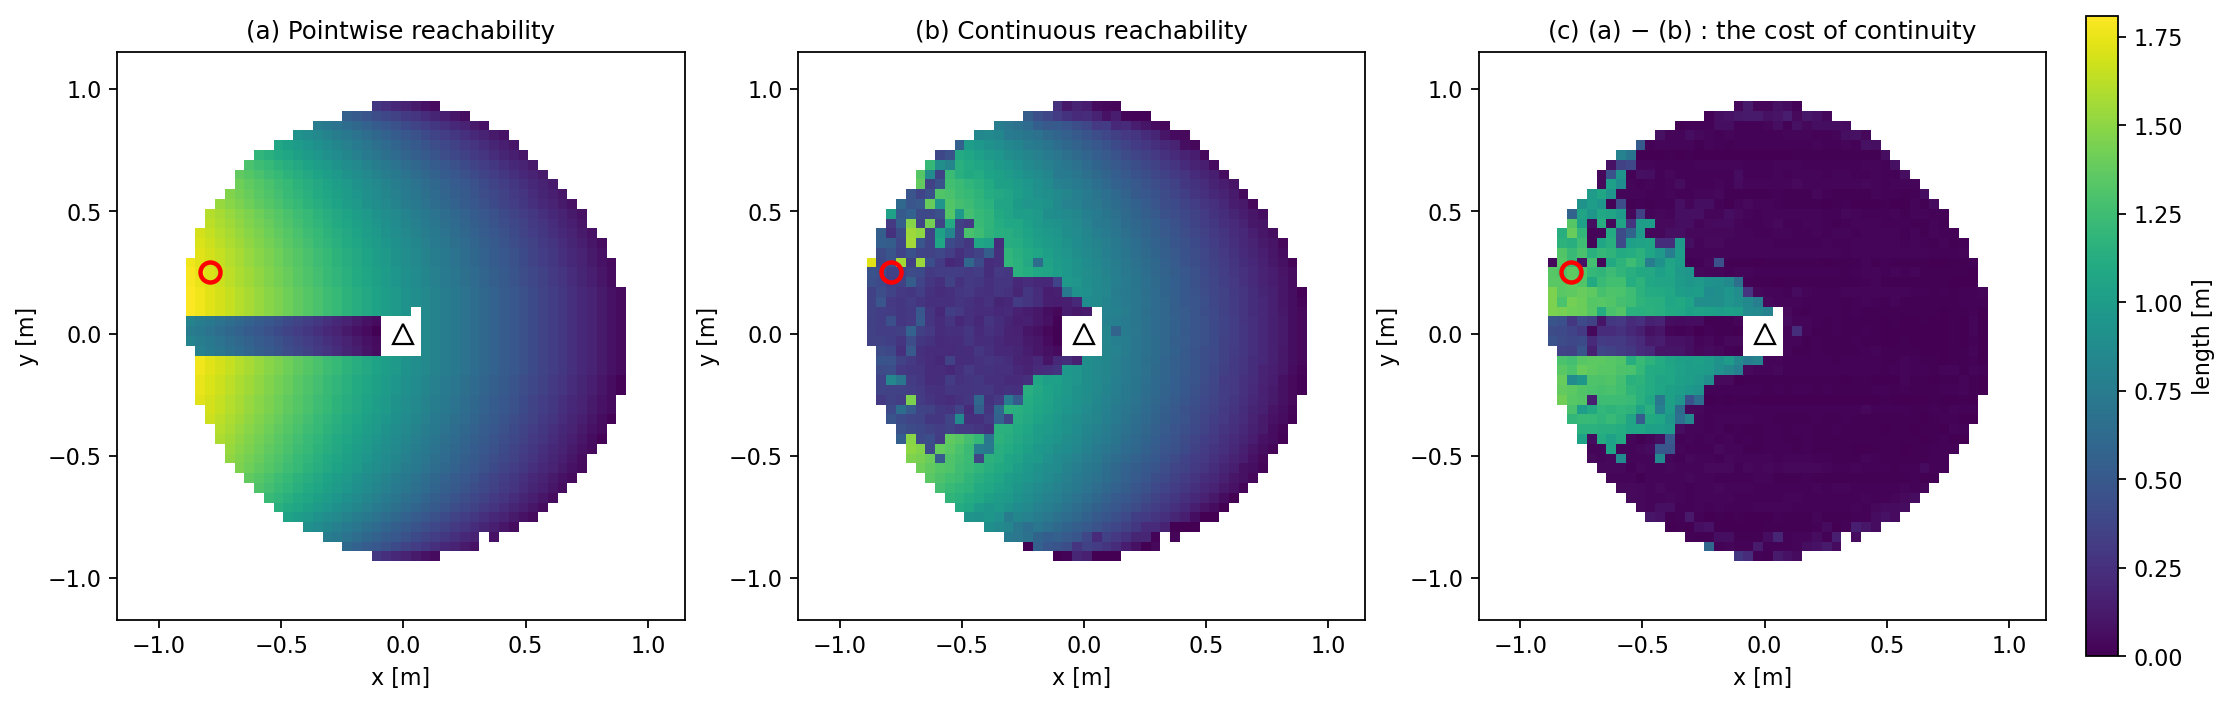
\includegraphics[width=\linewidth]{imgs/motivation_fig.png}
    \caption{Pointwise reachability overestimates continuous reachability. From each point on the plane $z=0.2\,\mathrm{m}$, the tool moves along $+x$ under a $30^\circ$ orientation cone and self-collision constraints. (a) Farthest distance with pointwise-valid configurations. (b) Farthest distance achievable by a single continuous joint trajectory. The median achievable path length decreases from $0.71\,\mathrm{m}$ to $0.46\,\mathrm{m}$. White cells denote infeasible starts. \new{The two panels differ only in whether the configurations along the path are required to be connected by one continuous joint trajectory, so the gap between them is the part of the reachability that pointwise analysis reports but no single stroke delivers. Closing that gap is what the two-stage framework of this paper is for.}\xinyitodo{这张图讲连续可达性和单点可达性的区别，然后点出来我们是通过两阶段方法，来尽量通过连续可达性兑现单点可达性。可以包含机械臂的图片，渲染图切片}}
    \label{fig:pwgap}
\end{figure}

\new{As Fig.~\ref{fig:motivation} makes concrete, the outcome of an extended
stroke is decided by two coupled choices, neither of which a reachability map
sees. The first is made once, before the motion begins: which branch of the
task-feasible configuration set the stroke starts on --- a discrete choice that
no continuous motion can revise afterwards. The second is made at every control
step: how the kinematic redundancy is resolved, since the joint motion chosen
now steers which constraint the arm will meet tens of increments later. The
problem is therefore a long-term decision problem in which the horizon itself
--- when the stroke ends --- is the quantity being optimized. Its natural
formal home is a discounted \emph{exit-time} optimal control problem, and this
paper builds the solution directly on that structure.}

\new{The exit-time formulation pays off twice. First, its Hamilton--Jacobi--Bellman
(HJB) equation is affine in the box-bounded null-space command, so the optimal
redundancy resolution reduces, without loss, to \emph{switching among the
$2^{m}$ vertices} of the command box, governed by the sign pattern of
$\mathbf{G}^{\!\top}\nabla V$ --- an orthant choice, not a magnitude
(Section~\ref{sec:hjb}). Second, it identifies exactly what the classical
null-space law gets wrong: the classical law reads the gradient of a
hand-weighted instantaneous surrogate, whereas the optimal law reads the
gradient of future feasible progress. Substituting the analytically available
\emph{constraint-margin field} --- a soft minimum of the normalized joint-limit
and orientation-cone margins --- for the intractable $V$ turns this analysis
into a deployable resolution law: training-free, one gradient evaluation per
step, and, as the experiments show, already at the level that exact
receding-horizon optimization of the same objective attains. The remaining
decision, the branch to start from, is where learning earns its place: the
achievable strokes of candidate starts differ by hundreds of millimeters, a
signal far above what a network can resolve, and their labels are generated for
free by rolling each candidate under the same analytic law. A permutation-equivariant
selector, conditioned on a sampled table of the path ahead, makes that choice
in one forward pass and generalizes to path families it was never trained on.}

\new{We evaluate the framework on path-following tasks across three
manipulators, measuring the achieved path length against the pointwise-reachable
length of the same task, so that the reported fraction is bounded by
construction and the gap between pointwise and continuous reachability is
itself quantified. A ladder of solution strategies for the same exit-time
problem --- from no null-space motion, through the classical law, to exact
receding-horizon optimization --- locates the analytic margin law at the top of
the ladder at a fraction of the optimization cost, with learned policies
included as baselines. The selector is evaluated in and out of its training
distribution: trained on straight and constant-curvature tasks, tested on
serpentine and non-planar families it has never seen. We further examine
cross-manipulator replication, executability of the switching strokes, and
base placement.}

\new{An earlier and shorter version of this work, restricted to one manipulator,
using a generative model for the initial configuration, a learned trajectory
stage, and reporting lengths against a best-of-$K$ reference, is available as a
preprint~\cite{yuan2026extreme}. This article differs from it in the
measurement itself, which is the point of departure for everything below; in
the trajectory stage, which is here derived analytically from the exit-time
structure rather than trained; and additionally in the candidate layer, in the
number of manipulators, and in the generalization and placement studies.}

\new{The contributions are as follows.}
\begin{itemize}
\item \new{\textbf{An exit-time optimal-control characterization of extreme
motion generation, and the resolution law it yields.} Maximizing the feasible
extent is cast as a discounted exit-time problem whose HJB Hamiltonian is
affine in the box-bounded null-space command. The greedy policy with respect
to \emph{any} differentiable value estimate can therefore be taken on the
$2^{m}$ vertices of the command box --- redundancy resolution is an orthant
choice, not a magnitude --- and the classical law is absorbed into the same
family as the gradient of an instantaneous surrogate read with its magnitude.
Substituting the analytically available constraint-margin field for the
value function converts the characterization into a deployable law:
training-free, one gradient evaluation per step, matching exact
receding-horizon optimization of the same objective, and transferring across
three manipulators of different morphology without retuning.}
\item \new{\textbf{A verified two-sided bracket of continuous kinematic
reachability, and the measurement it yields.} Reporting stroke length against
the longest of $K$ sampled candidates, as our earlier version
did~\cite{yuan2026extreme}, is not sound: we show that achieved strokes exceed
such a reference. We instead reference each task by marching along its own
path and testing whether any admissible configuration exists at each sample;
the result depends on the kinematics and the feasibility search alone, and its
validity as a bound is itself checked --- no executed stroke exceeds it, and
it is stable when the search budget is doubled. Between this upper reference
and the executed stroke as the lower one, the gap between pointwise and
continuous reachability is quantified per task, across three manipulators and
over a distribution of tasks. Because a query is cheap, the same measurement
can be swept over thousands of base poses, which corrects a systematic
optimism in reachability-map-based placement.}
\item \new{\textbf{A selector for the one decision a resolution law cannot
make, with supervision that costs nothing.} How far a stroke reaches is
decided first by which branch of the task-feasible configuration set it starts
on --- a discrete choice no continuous resolution can revise once the motion
has begun, and one that no quantity computable at the start of the stroke
predicts. We supervise the choice on the outcome itself, rolling every
candidate to termination \emph{under the analytic law}, so the labels require
no training and no human annotation. The score is permutation-equivariant
over the candidate set and conditioned on a sampled table of the path ahead;
trained on straight and constant-curvature tasks alone, it transfers to
serpentine and non-planar families it has never seen.}
\item \new{\textbf{A measured division of labor between learning and
analysis.} The two stages consume differences of different magnitude:
across candidate starts, achievable strokes differ by hundreds of millimeters
and their values are learnable; within one configuration, the one-step margin
differences that separate the $2^{m}$ vertices are two orders of magnitude
smaller, and exactly there the analytic gradient supplies the answer in closed
form. Placing learning at the selection layer and analysis at the control
layer is therefore not a preference but a consequence of the measured scales,
established by controlled probes at both layers.}
\end{itemize}

\section{Related Work}

Extreme motion generation is essentially related to the manipulator's reachable workspace and local motion dexterity during motion execution. Manipulability and reachability describe local instantaneous motion dexterity and global spatial feasibility, respectively. However, neither measure indicates how joint-space motion should be coordinated to approach the boundary of the reachable workspace along a continuously executable path.

\subsection{Manipulability}
The manipulability ellipsoid \cite{yoshikawa1985manipulability} characterizes the local relationship between joint-space and task-space velocities through the Jacobian. Intuitively, the ellipsoid volume captures overall dexterity, while its projection along a task direction quantifies directional motion capability. Subsequent work extended this description to dynamic and task-specific settings.

The local measurement was subsequently extended to account for task and dynamic requirements. For example, Yoshikawa~\cite{yoshikawa1985dynamic} introduced the dynamic manipulability to characterize achievable end-effector accelerations under joint force limits. Chiu~\cite{chiu1988task} further proposed a task-compatibility measure for evaluating manipulator configurations against directional velocity and force requirements. Klein and
Blaho~\cite{klein1987dexterity} systematically compared several local dexterity measures and revealed that different indicators emphasize distinct capabilities and may lead to different optimal configurations. Beyond ellipsoidal indices, Chiacchio et al.~\cite{chiacchio1997force} introduced task-space force polytopes for redundant manipulators, and Skuric et al.~\cite{skuric2021line} adapted the online calculation. Despite these expansions, the above measures characterize capability at a given joint configuration rather than considering its evolution along a continuous path.

Manipulability has been incorporated into both redundancy resolution and motion planning. Liegeois et al.~\cite{liegeois1977automatic} established the null-space gradient-projection framework for optimizing secondary objectives while ensuring the primary task requirements. Jin et al.~\cite{jin2017manipulability} adopted a dynamic neural network for inverse-free manipulability optimization; Jaquier et
al.~\cite{jaquier2021geometry} developed a geometry-aware controller for tracking learned manipulability profiles. More recently, Haviland and
Corke~\cite{haviland2021neo} incorporated manipulability maximization into
reactive optimization-based control. Manipulability can also guide motion planning. Shen et al.~\cite{shen2023adaptive} proposed a manipulability-aware $\text{RRT}^{\star}$ that incorporates the measure into both the planning cost and step size, while Cai et al.~\cite{cai2025just} balanced path cost against manipulability to mitigate singularities. Although these methods significantly extend the path length through improving local dexterity, the factors that lead to maximum continuously executable path length remain unexplored.

\subsection{Reachability and Global Redundancy Resolution}
Complementary to local dexterity, workspace reachability characterizes the global spatial feasibility of a manipulator. Early studies developed
geometric criteria and capability maps to represent reachable task-space
regions~\cite{yang2009placement,zacharias2007capturing}. The reachability was subsequently utilized for manipulator base placement optimization \cite{makhal2018reuleaux, vahrenkamp2013robot}. More recently, Feng et al.~\cite{feng2025predictive} introduced predictive reachability via world models for embodiment selection, while Jauhri et al.~\cite{jauhri2022robot} used reachability priors to accelerate RL-based control, and Selim et al.~\cite{selim2022safe} proposed a reachability-based safety layer with formal guarantees. Despite these advances, workspace reachability remains region-level descriptions indicating where valid configurations exist. However, they lack guidance on how those configurations can be reached through a single continuously feasible motion toward the reachable boundary.

Beyond describing the reachable workspace as a spatial envelope, another line
of work examines the global structure of the inverse-kinematic solution set and
its implications for continuous motion. Burdick~\cite{burdick1989inverse}
showed that the infinite IK solutions of a redundant manipulator form a
finite family of disjoint continuous self-motion manifolds. For 7-DoF
manipulators, Shimizu et al.~\cite{shimizu2008analytical} further showed that
joint limits partition the feasible arm-angle domain into multiple disconnected
intervals and proposed to select a favorable branch for avoiding joint limits in redundancy resolution. Hauser and Emmons~\cite{hauser2018global} formulated global redundancy resolution as the construction of a continuous pseudoinverse of the forward-kinematic map, while Ferrentino and Chiacchio~\cite{ferrentino2020optimal} developed a dynamic-programming-based method to compute globally optimal joint-space paths across different path-homotopy classes and self-motion manifolds. Although these methods reason over the global solution set and the entire path planning, they still treat the Cartesian path as pre-defined. Therefore, they mainly address how a prescribed path can be optimally executed rather than how far it can be extended before avoiding kinematic constraints. This leaves open the complementary problem addressed in this work: jointly selecting the initial configuration and resolving redundancy to maximize the feasible Cartesian stroke.


% \subsection{Learning-based Motion Generation}
\subsection{Learning-based Redundancy Resolution}
\new{Both families above resolve the redundancy by optimizing a quantity defined
at the current configuration. Learning-based methods instead fit a distribution
over feasible configurations and can therefore represent several resolutions of
the same pose at once. Reinforcement learning has been applied to redundancy
resolution~\cite{malik2022deep}, and generative solvers such as
IKFlow~\cite{ames2022ikflow} and IKDiffuser~\cite{zhang2025ikdiffuser} model the
full solution set rather than returning one solution.
DiffusionSeeder~\cite{huang2024diffusionseeder} uses a generative model to seed
downstream trajectory optimization, and Yoon et al.~\cite{yoon2023learning}
learn an initialization for path-following problems. These works confirm that
the multiplicity of solutions is worth modeling, but they are evaluated by how
well a prescribed path is executed, not by how far a path can be extended before
execution becomes infeasible.}

\new{This paper draws the line between learning and analysis differently from
this literature, and by measurement rather than by preference. The quantity a
within-stroke resolution law must discriminate --- which of the $2^{m}$
extreme null-space directions preserves the most future margin --- is
available in closed form as a gradient, while the quantity the initial-configuration
choice must discriminate --- which branch yields the longer stroke --- is
available only by rolling the stroke out. We therefore reserve learning for
the selection stage, where the signal is large and the labels are generated
by the analytic law itself, and evaluate learned within-stroke policies
(continuous and vertex-valued, with and without a classical supervisor) as
baselines under identical conditions in Section~\ref{sec:setup}.}


\subsection{\new{Quantifying Continuous Reachability}}
\new{Two lines of work are close enough to this paper that the differences must
be stated precisely. The first asks whether a prescribed path can be executed at
all by one continuous joint trajectory. Hauser~\cite{hauser2016continuous}
formalizes a hierarchy of pointwise, pathwise and global redundancy resolution,
and Hauser and Emmons~\cite{hauser2018global} show, for a joint-limited planar
arm, interior workspace paths whose waypoints are individually reachable while
no continuous joint-space resolution exists; at the workspace level they report
the percentage of roadmap edges that remain disconnected. The same distinction
appears in the cuspidal-manipulator literature, where a region in which every
continuous path is feasible is called $t$-connected~\cite{wenger1991uniqueness,
wenger2023cuspidal}, and where it is stated plainly that a path may admit an
inverse-kinematic solution at every point and still have no continuous
joint-space realization~\cite{elias2025cuspidal}. These are set-valued or binary
statements: a region either has the property or it does not, an edge is either
traversable or not.}

\new{The second line measures how much of a path is covered when it cannot be
covered entirely, and does so with a count. IKLink~\cite{wang2024iklink} and
Yang et al.~\cite{yang2022optimal} minimize the number of reconfigurations
needed to track an end-effector trajectory, and Yin et
al.~\cite{yin2024breakpoints} minimize the number of breakpoints. A count of
interruptions answers how many times the motion must stop; it does not localize
the first failure, does not yield an arc length, and admits no upper bound
against which to read it. Because these formulations permit reconfiguration,
they also cannot ask how far a \emph{single} stroke reaches. Closest in spirit
is the base-placement work of Gautier et al.~\cite{gautier2024comparison}, which
reports the maximum weldable height and length attainable along prescribed
trajectories before a kinematic event intervenes; those figures are real-valued,
but they are case-study numbers for a non-redundant arm, terminated by
singularity, and one-sided, since nothing certifies that a longer stroke does
not exist.}

\new{Comparisons between resolution laws are older still. Suh and
Hollerbach~\cite{suh1987local} and Kazerounian and Wang~\cite{kazerounian1988global}
contrast local with globally optimal resolution and report the performance
ordering between them, and Martin et al.~\cite{martin1989resolution} observe
that extremal solutions fall into distinct homotopy classes of lifts of the
workspace path, not all of which are optimal, and note that each such solution
is nevertheless globally optimal \emph{within its own class}, so that sufficiency
conditions must consider the topology of those lifts. \new{Optimal resolution within one class is therefore long settled; what has
not been quantified is the outer choice among the classes.} Modern treatments search
across the classes rather than within
one~\cite{ferrentino2020optimal,ferrentino2021globally,fabregat2025topological}.
The discrete obstruction is therefore well known, and so is the fact that the
law matters. What is missing is an attribution: how much of the achievable
task-space extent is decided by which branch the arm starts on, as against the
law applied within it, measured over a distribution of tasks rather than on a
single pose or a single instance.}

\section{Problem Formulation}
While extreme motion generation applies broadly to constrained path following, we here specify it as extreme straight-line path following. Specifically, a fixed-base manipulator advances its end-effector along the line with a tool-orientation constraint. As illustrated in Fig.~\ref{overview}, solving this problem requires first determining the initial joint configuration from which the motion starts and then generating the motion that maximizes the achievable path length.

\begin{figure}[!htbp]
    \centering
    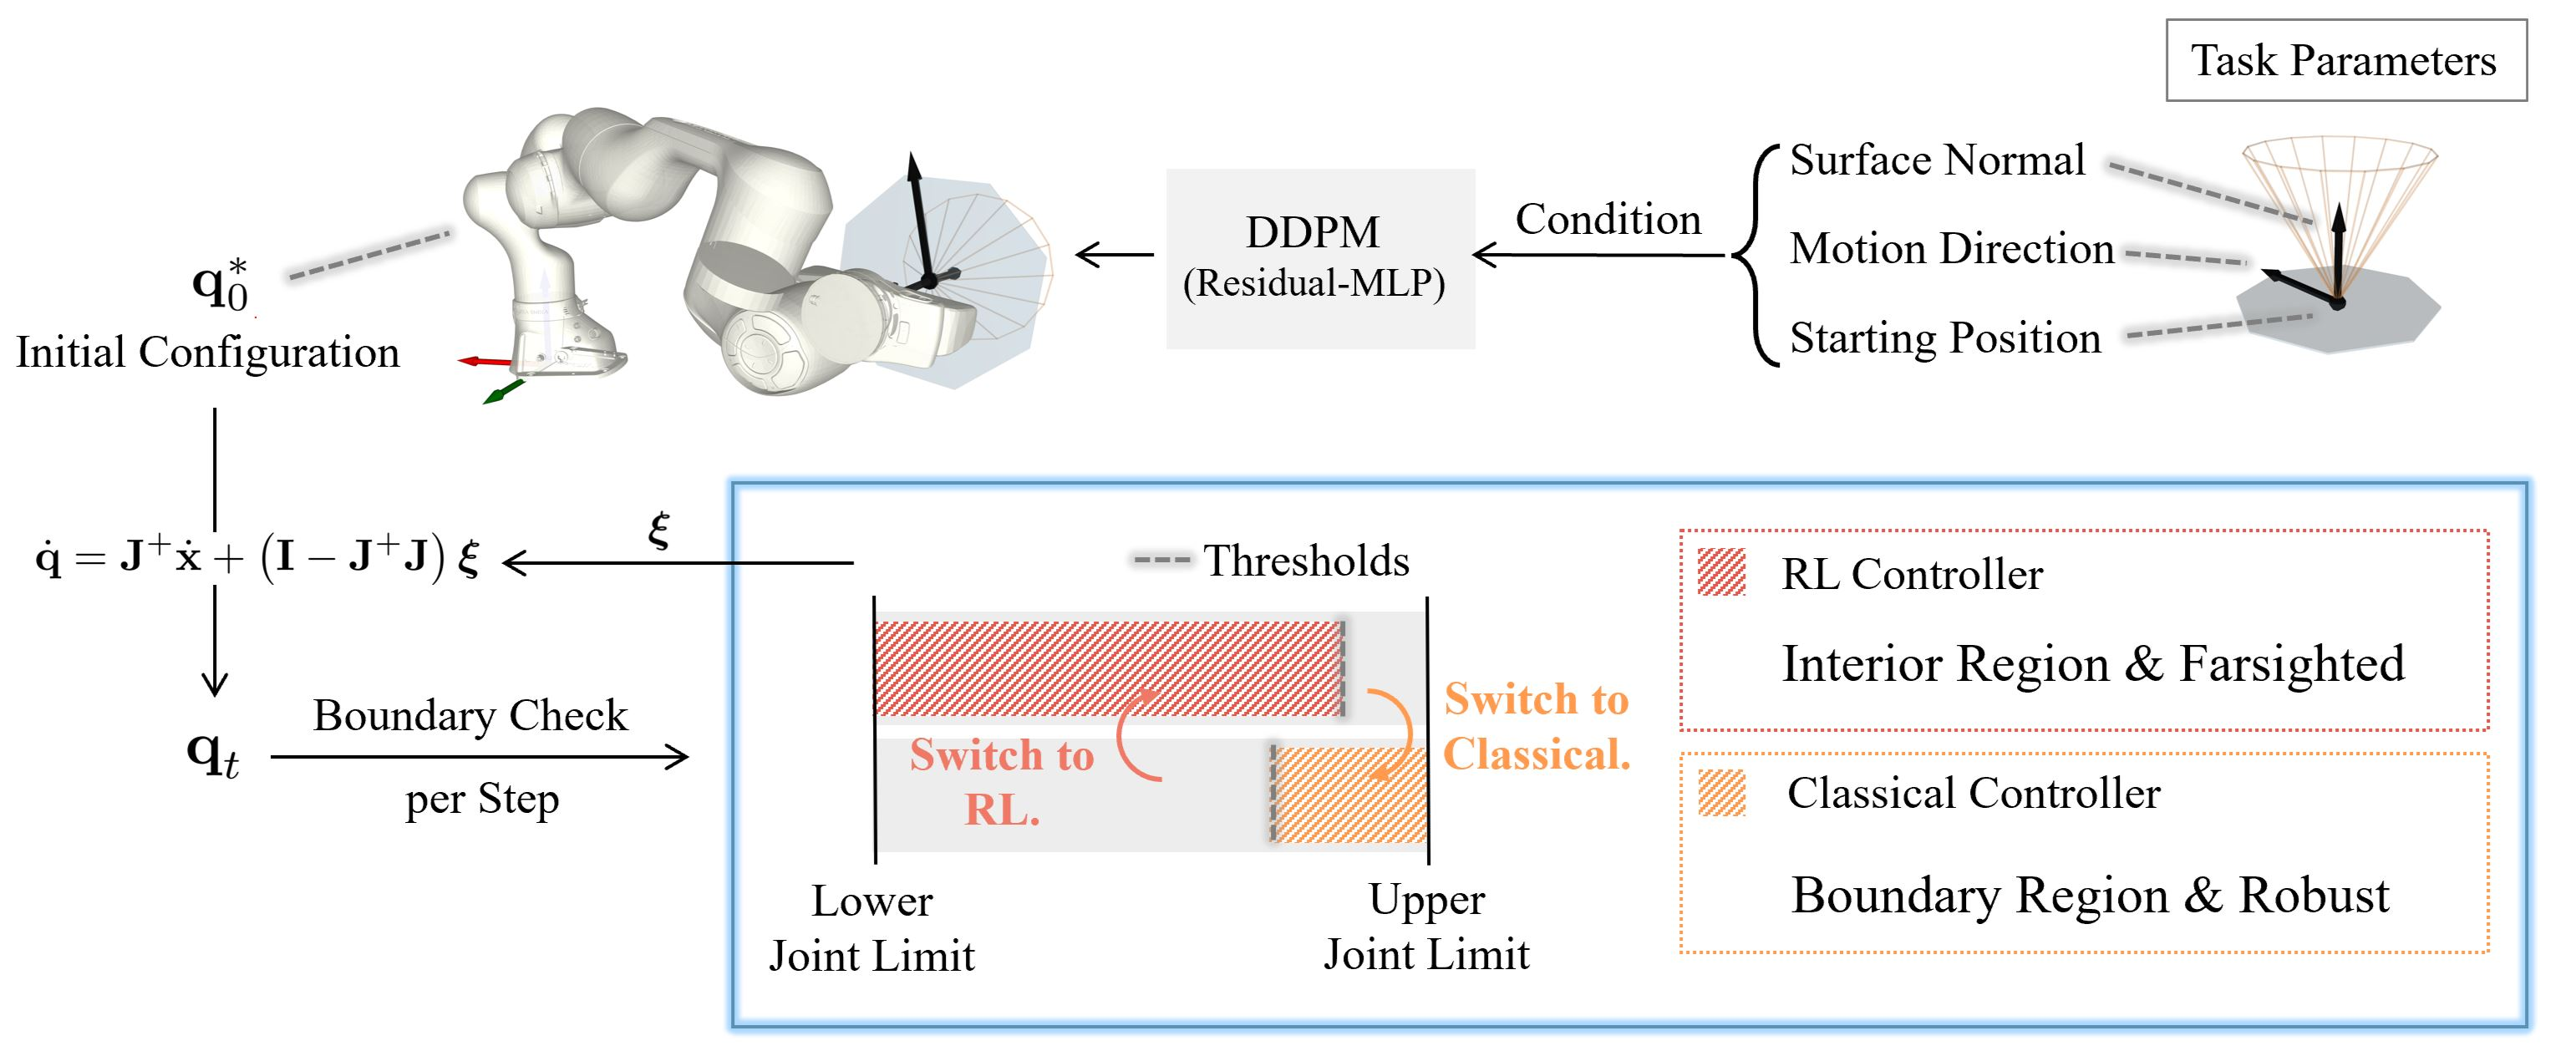
\includegraphics[width=\linewidth]{imgs/system_overview.JPG}
    \caption{Overview of the two-stage framework for extreme motion generation.}
    \label{overview}
\end{figure}

Formally, consider a manipulator with $n$ degrees of freedom, where $\mathbf{q} \in \mathbb{R}^{n}$ denotes the joint configuration. Let $\mathbf{p}(\mathbf{q}) \in \mathbb{R}^{3}$ denote the end-effector position and $\mathbf{z}(\mathbf{q}) \in \mathbb{R}^{3}$ denote the TCP local $z$-axis. A straight-line path-following task is specified by the condition vector:
\begin{equation}
\label{cond}
\mathbf{c} = [\mathbf{p}_{0}, \mathbf{d}, \mathbf{n}] \in \mathbb{R}^{9},
\end{equation}
where $\mathbf{p}_{0}$ denotes the starting position, and $\mathbf{d}$ and $\mathbf{n}$ are unit vectors representing the desired motion direction and task-plane normal, respectively. \new{The prescribed path is the ray $\mathcal{P}=\{\mathbf{p}_{0}+s\,\mathbf{d} : s\ge 0\}$, along which the end-effector advances at a commanded speed $v$, one command being issued per control period $\Delta t$.} \new{The straight ray is the default member of a family of paths sharing this
condition vector: prescribing a signed curvature $\kappa$ bends the ray into a
constant-curvature arc in the plane spanned by $\mathbf{d}$ and
$\mathbf{n}\times\mathbf{d}$; a lateral offset $A\sin(2\pi s/\lambda)$ turns it
into a serpentine seam; and letting the cone axis $\mathbf{n}(s)$ rotate with
arc length models a non-planar workpiece. All four families are evaluated in
Section~\ref{sec:setup}; the formulation below is written for the ray and
carries over unchanged, with $\mathbf{d}$ read as the instantaneous tangent
and $\mathbf{n}$ as the local cone axis.}

Starting from an initial configuration $\mathbf{q}_{0}^{*}$, the policy $\pi$ determines the joint motion at every control step to maximize the executed path length, producing a joint trajectory $\{\mathbf{q}_{t}^{*}\}_{t=0}^{T}$ initialized at $\mathbf{q}_{0}^{*}$, where $T$ is the termination step at which any safety constraint is first violated. \new{The executed motion is called a \emph{stroke}, and its Cartesian length is the stroke length $\mathcal{L}$.} This task can be formalized as a constrained optimization problem as:
\begin{align}
\max_{\mathbf{q}_{0}^{*},\,\pi} \quad & \mathcal{L}(\mathbf{q}^{*}_{0},\,\pi;\,\mathbf{p}_{0}, \mathbf{d}, \mathbf{n}) \\
\text{s.t.} \quad & {\color{red}\operatorname{dist}\bigl(\mathbf{p}(\mathbf{q}_{t}^{*}),\,\mathcal{P}\bigr) \leq \epsilon_{\text{pos}}}, \label{eq:pos_constraint} \\
& \arccos\!\left( \mathbf{z}(\mathbf{q}_{t}^{*})^{\top} \mathbf{n} \right) \leq \theta_{\max}, \label{eq:ori_constraint} \\
& \mathbf{q}_{\min} \preceq \mathbf{q}_{t}^{*} \preceq \mathbf{q}_{\max}, \label{eq:jl_constraint}
\end{align}
where $\mathcal{L}$ denotes the stroke length, $\mathbf{q}_0^*$ and $\pi$ are the initial configuration and the control policy to be optimized, and $(\mathbf{p}_0, \mathbf{d}, \mathbf{n})$ specify the task conditions as above. The $\epsilon_{\text{pos}}$, $\theta_{\max}$, and $[\mathbf{q}_{\min}, \mathbf{q}_{\max}]$ are the position tolerance, orientation tolerance, and joint limits, respectively.

During this process, since only the $3$-DoF end-effector position must be precisely tracked, the remaining freedom makes the manipulator kinematically redundant for $n>3$. This redundancy is resolved in the null space of the position Jacobian, which decomposes the commanded joint velocity into a task term and a null-space term,
\begin{equation}
\label{eq:nullspace}
{\color{red}
\dot{\mathbf{q}} = \mathbf{J}^{+}_{\lambda}\dot{\mathbf{x}} + \mathbf{B}(\mathbf{q})\,\mathbf{u},
\qquad
\mathbf{J}\mathbf{B}=\mathbf{0},\quad
\mathbf{B}^{\!\top}\mathbf{B}=\mathbf{I},}
\end{equation}
\new{where $\mathbf{J}^{+}_{\lambda}$ is the damped pseudo-inverse of the position Jacobian $\mathbf{J}$, $\mathbf{B}(\mathbf{q})\in\mathbb{R}^{n\times(n-3)}$ is an orthonormal basis of the exact null space of $\mathbf{J}$ (identified by a double-precision SVD; its task-aligned construction is given in Section~\ref{sec:traj}), and $\mathbf{u}$ collects the null-space coordinates of the secondary motion. The exact basis, rather than the projector $(\mathbf{I}-\mathbf{J}^{+}_{\lambda}\mathbf{J})$, matters here: with a damped pseudo-inverse that matrix is not an exact projector, whereas $\mathbf{J}\mathbf{B}=\mathbf{0}$ holds by construction, so the secondary motion cannot disturb the end-effector position regardless of the damping.} Within this null space, several secondary objectives can be pursued:
\begin{equation}
\label{eq:secondary}
\boldsymbol{\xi}=k_{\mu}\,\nabla_{\mathbf{q}}w_{\mathbf{d}}(\mathbf{q})\;-\;k_{\mathrm{jl}}\,\frac{\mathbf{q}-\mathbf{q}_{\mathrm{mid}}}{\mathbf{q}_{\max}-\mathbf{q}_{\min}}\;+\;k_{\theta}\,g(\theta)\,\nabla_{\mathbf{q}}\!\big(\mathbf{z}(\mathbf{q})^{\top}\mathbf{n}\big),
\end{equation}
where the secondary field $\boldsymbol{\xi}$ combines a directional-manipulability term $w_{\mathbf{d}}$ that retreats from singularities along $\mathbf{d}$, a centering term that pulls each joint toward the middle $\mathbf{q}_{\mathrm{mid}}$ of its range, and a cone term gated by $g(\theta)$ that activates only as the tool axis approaches the $\theta_{\max}$ boundary. \new{The classical law enters the decomposition through its null-space coordinates, $\mathbf{u}\propto\mathbf{B}^{\!\top}\boldsymbol{\xi}$ up to the gain scaling and a saturation; all subsequent controllers share Eq.~(\ref{eq:nullspace}) and differ only in how $\mathbf{u}$ is generated.}

{\color{red}
The horizon of this problem is not an input: the stroke ends at the first
constraint violation, and when that happens is itself decided by the commands
being optimized. The natural formal home for such an objective is an
\emph{exit-time} optimal control problem. We state it here;
Section~\ref{sec:hjb} derives from it the structure that the rest of the paper
builds on.

Collect the constraints of
Eqs.~(\ref{eq:pos_constraint})--(\ref{eq:jl_constraint}), together with the
self-collision clearance, into an open feasible set $\Omega$ of configurations,
and let
\begin{equation}
\label{eq:exit}
\tau \;=\; \inf\bigl\{\,t \ge 0 \;:\; \mathbf{q}(t) \notin \Omega \,\bigr\}
\end{equation}
denote the exit time of a closed-loop trajectory (not to be confused with the
dimensionless switching thresholds $\tau_{\mathrm{enter}},\tau_{\mathrm{exit}}$
of Section~\ref{sec:traj}). Throughout this work the null-space coordinates
are bounded, $\mathbf{u} = a_{\max}\,\mathbf{a}$ with
$\mathbf{a} \in \mathcal{A} := [-1,1]^{m}$, where $m = n-3$ is the dimension
of the null space left by the position task ($m=4$ for the two 7-DoF arms,
$m=3$ for Cobotta). Under this bound the decomposition of
Eq.~(\ref{eq:nullspace}) is control-affine,
\begin{equation}
\label{eq:affine}
\dot{\mathbf{q}} \;=\; \mathbf{f}(\mathbf{q}) \;+\; \mathbf{G}(\mathbf{q})\,\mathbf{a},
\qquad
\mathbf{f} := \mathbf{J}^{+}_{\lambda}\dot{\mathbf{x}},\quad
\mathbf{G} := a_{\max}\,\mathbf{B},
\end{equation}
with the task condition $\mathbf{c}$ entering $\mathbf{f}$ and $\Omega$ as a
fixed parameter. Writing $r(\mathbf{q}) \ge 0$ for the instantaneous advance
rate along $\mathbf{d}$ --- the continuous-time counterpart of the reward
defined in Section~\ref{sec:traj} --- define the discounted progress value
\begin{equation}
\label{eq:value}
V(\mathbf{q}_{0}) \;=\; \sup_{\mathbf{a}(\cdot)}
\int_{0}^{\tau} e^{-\beta t}\, r(\mathbf{q}(t))\,\mathrm{d}t,
\end{equation}
where the supremum runs over measurable commands into $\mathcal{A}$ and the
discount $\beta > 0$ matches the implementation ($\gamma = 0.99$ at a $50$\,ms
control period gives $\beta = -\ln\gamma/\Delta t \approx 0.2\,\mathrm{s}^{-1}$). On
the straight-line family the task term of Eq.~(\ref{eq:nullspace}) holds the
advance rate at the commanded speed $v$ up to the damping-induced tracking
error, so $r \approx v$ and
$V \approx (v/\beta)\bigl(1 - e^{-\beta\tau}\bigr)$ is an increasing function
of the exit time alone: on this family the discounted problem is a
maximum-exit-time problem. $V$ in (\ref{eq:value}) is the optimal value; the
learned component of this paper approximates the value of a \emph{policy}:
the selector is supervised by rollouts of the deployed closed loop --- the
analytic law of Section~\ref{sec:relation} --- so it ranks candidates by that
loop's $V^{\pi}$, not by $V$ (the critics of the learned baseline policies
likewise regress their own $V^{\pi}$). The two decision variables of the
constrained program above reappear as the two stages of the framework: the
selection stage chooses $\mathbf{q}_{0}^{*}$ by that ranking across the
disconnected components of the feasible set, and the trajectory stage resolves
the redundancy at every increment in pursuit of the same objective.

Two facts about this formulation are properties of the system as constructed,
not modeling assumptions, and they are all that the analysis of
Section~\ref{sec:hjb} uses. First, the dynamics (\ref{eq:affine}) are affine
in $\mathbf{a}$ by the definition of the null-space decomposition. Second,
the advance rate $r$ does not depend on $\mathbf{a}$, because
$\mathbf{J}\mathbf{B}=\mathbf{0}$ holds exactly in
Eq.~(\ref{eq:nullspace}): the damping enters only the particular solution.
What separates the exit-time form from instantaneous null-space optimization
is therefore the argument of the maximization alone: a command at $\mathbf{q}$
is judged by how it changes all future feasible progress, through $V$, and not
by any quantity evaluable at $\mathbf{q}$ in isolation.
}

% \subsection{Task Optimization via Null-Space Control}
% \wan{零空间控制属于常识，有必要做前提知识吗？}\xinyi{可删除章节。}\wan{把下一节开头的任务具化放在这里，具化完后简单讲一下零空间。}
% \label{sec:baseline}
% % here to state how is the joint velocity be decomposed, and how is the null space been improved via gradient asent. List the fomulars. the detailed formulas can be put in the appendix
% For a manipulator, the position Jacobian $\mathbf{J}(\mathbf{q})=\partial\mathbf{p}/\partial\mathbf{q}\in\mathbb{R}^{3\times n}$ has a non-trivial null space, so the joint velocity that realizes a desired end-effector motion is not unique. The classical law decomposes the commanded joint velocity into a task term and a null-space term,
% \begin{equation}
% \label{eq:nullspace}
% \dot{\mathbf{q}} = \mathbf{J}^{+}\dot{\mathbf{x}} + \big(\mathbf{I}-\mathbf{J}^{+}\mathbf{J}\big)\,\boldsymbol{\xi},
% \end{equation}
% where $\mathbf{J}^{+}=\mathbf{J}^{\top}(\mathbf{J}\mathbf{J}^{\top}+\lambda^{2}\mathbf{I})^{-1}$ is the damped pseudo-inverse with a Nakamura--Hanafusa adaptive damping $\lambda$ that grows only as the smallest singular value of $\mathbf{J}$ drops below a threshold, and $\mathbf{I}-\mathbf{J}^{+}\mathbf{J}$ projects the secondary command $\boldsymbol{\xi}$ onto the null space. 

% For the straight-line path following task in this study, the task velocity $\dot{\mathbf{x}}=v\,\mathbf{d}+\mathbf{K}_{P}(\mathbf{p}_{\mathrm{ref}}-\mathbf{p})$ advances the end-effector along the line at speed $v$ while a proportional term rejects lateral drift from the reference point $\mathbf{p}_{\mathrm{ref}}$ on the line\footnote{In the ideal case, the task decomposition in Eq.~(\ref{eq:nullspace}) keeps the end-effector exactly on the primary task. In practice, however, accumulated numerical errors cause gradual drift, which the proportional term $\mathbf{K}_{P}(\mathbf{p}_{\mathrm{ref}}-\mathbf{p})$ corrects.}. The secondary command performs gradient ascent on a weighted sum of redundancy objectives,
% \begin{equation}
% \label{eq:secondary}
% \boldsymbol{\xi}=k_{\mu}\,\nabla_{\mathbf{q}}w_{\mathbf{d}}(\mathbf{q})\;-\;k_{\mathrm{jl}}\,\frac{\mathbf{q}-\mathbf{q}_{\mathrm{mid}}}{\mathbf{q}_{\max}-\mathbf{q}_{\min}}\;+\;k_{\theta}\,g(\theta)\,\nabla_{\mathbf{q}}\!\big(\mathbf{z}(\mathbf{q})^{\top}\mathbf{n}\big),
% \end{equation}
% combining a directional-manipulability term $w_{\mathbf{d}}$ that retreats from singularities along $\mathbf{d}$, a centering term that pulls each joint toward the middle $\mathbf{q}_{\mathrm{mid}}$ of its range, and a cone term gated by $g(\theta)$ that activates only as the tool axis approaches the $\theta_{\max}$ boundary.



\section{\texorpdfstring{\new{HJB Structure and Vertex-Valued Feedback}}{HJB Structure and Vertex-Valued Feedback}}
\label{sec:hjb}

{\color{red}
This section derives what the exit-time formulation implies about the
structure of the optimal secondary command. Three conclusions build on one
another: the command box $\mathcal{A}$ can be replaced by its $2^{m}$
vertices without loss; the classical law of Eq.~(\ref{eq:secondary}) belongs
to the same family of controllers as the optimal one, differing in two
identifiable substitutions; and reversing the two substitutions with an
analytically available scalar field yields the resolution law this paper
deploys.

\subsection{HJB Characterization}
At points of differentiability, the value function (\ref{eq:value}) satisfies
the Hamilton--Jacobi--Bellman (HJB) relation of the discounted exit-time
problem,
\begin{equation}
\label{eq:hjb}
\beta V \;=\; r \;+\; \nabla V^{\!\top}\mathbf{f}
\;+\; \sup_{\mathbf{a}\in\mathcal{A}}
\bigl(\mathbf{G}^{\!\top}\nabla V\bigr)^{\!\top}\mathbf{a},
\qquad V \equiv 0 \ \text{outside } \Omega .
\end{equation}
Because $r$ and $\mathbf{f}$ do not depend on $\mathbf{a}$, the command enters
only through the last term, linearly. Define the \emph{switching vector}
\begin{equation}
\label{eq:sigma}
\boldsymbol{\sigma}(\mathbf{q}) \;:=\;
\mathbf{G}(\mathbf{q})^{\!\top}\nabla V(\mathbf{q}) \;\in\; \mathbb{R}^{m},
\end{equation}
whose $i$-th component is the marginal effect of the $i$-th null-space
direction on discounted future feasible progress --- the long-horizon
counterpart of the instantaneous objective gradients of
Eq.~(\ref{eq:secondary}). The supremum in (\ref{eq:hjb}) equals
$\|\boldsymbol{\sigma}\|_{1}$ and, wherever no component of
$\boldsymbol{\sigma}$ vanishes, it is attained at the single vertex
$\mathbf{a} = \operatorname{sgn}\boldsymbol{\sigma}$. The redundancy
resolution implied by the value function is a switching controller: it
selects an orthant, not a magnitude.

\subsection{Lossless Vertex Reduction}
The observation above does not require $V$ to be the optimal value function;
it holds for the gradient field of any scalar function of the configuration,
which is what makes it usable by a learner whose value estimate is never
exact.

\begin{proposition}
\label{prop:vertex}
Let $W:\Omega\to\mathbb{R}$ be differentiable and
$\boldsymbol{\sigma}_{W} := \mathbf{G}^{\!\top}\nabla W$. Then, at every
$\mathbf{q}$,
\begin{equation}
\label{eq:prop}
\max_{\mathbf{a}\in[-1,1]^{m}} \boldsymbol{\sigma}_{W}^{\!\top}\mathbf{a}
\;=\;
\max_{\mathbf{a}\in\{-1,1\}^{m}} \boldsymbol{\sigma}_{W}^{\!\top}\mathbf{a}
\;=\; \|\boldsymbol{\sigma}_{W}\|_{1},
\end{equation}
attained at $\mathbf{a}=\operatorname{sgn}\boldsymbol{\sigma}_{W}$, with the
components on which $\sigma_{W,i}=0$ chosen arbitrarily in $\{-1,1\}$.
Consequently the greedy policy with respect to any differentiable value
estimate can be taken vertex-valued: the vertex action space is closed under
policy improvement.
\end{proposition}

\begin{IEEEproof}
$\boldsymbol{\sigma}_{W}^{\!\top}\mathbf{a}
= \sum_{i}\sigma_{W,i}\,a_{i} \le \sum_{i}|\sigma_{W,i}|$ for
$\mathbf{a}\in[-1,1]^{m}$, with equality iff
$a_{i}=\operatorname{sgn}\sigma_{W,i}$ on every component with
$\sigma_{W,i}\neq 0$; such an $\mathbf{a}$ can be chosen in $\{-1,1\}^{m}$.
\end{IEEEproof}

Three remarks delimit what the proposition does and does not say.

\begin{remark}[Value equivalence is conditional]
\label{rem:value}
Since the pointwise Hamiltonians of the box- and vertex-constrained problems
coincide by (\ref{eq:prop}), the two problems share their HJB equation; if,
in addition, the value function is characterized as the unique viscosity
solution of (\ref{eq:hjb}), then $V_{\mathrm{box}} = V_{\mathrm{vertex}}$.
The comparison conditions this requires are delicate for a nonsmooth feasible
set such as ours, and we neither verify nor use them.
\end{remark}

\begin{remark}[No bang-bang claim]
\label{rem:bangbang}
Where components of $\boldsymbol{\sigma}$ vanish, the maximizer in
(\ref{eq:hjb}) is not unique, so the accurate statement is that an optimal
vertex-valued \emph{selector exists}, not that every optimal command is a
vertex. The reduction is moreover exact in continuous time only: over a
finite control period the flow under a held command is no longer affine in
$\mathbf{a}$, so a vertex command held for $\Delta t$ can be strictly worse
than an interior one. The size of this finite-rate gap is an empirical
question, which Section~\ref{sec:setup} answers by sweeping the control
period.
\end{remark}

\begin{remark}[The command box is a design choice]
\label{rem:box}
The box $\mathcal{A}$ is defined in the constructed basis $\mathbf{B}$, in
the manner of per-direction rate limits; its vertex set is tied to that
basis. A ball constraint on the secondary command would instead yield the
full-magnitude solution $\mathbf{a}\propto\boldsymbol{\sigma}$ with no vertex
structure. The analysis is exact for the system as defined and claims no
canonical status for the box. The constructed basis can moreover change
discontinuously with $\mathbf{q}$ (the fallback branches of its
task-aligned construction, Section~\ref{sec:traj}), one more reason
Remark~\ref{rem:value} remains conditional.
\end{remark}

The structural conclusion has a precedent in a different corner of robotics:
in time-optimal control along a prescribed path, the torque box together with
control-affine dynamics forces the optimal path acceleration to the boundary
of the admissible set except on singular
arcs~\cite{bobrow1985time,shin1985minimum}. Proposition~\ref{prop:vertex} is
the kinematic counterpart of that mechanism for redundancy resolution.

\subsection{From the Classical Law to the Analytic Margin Law}
\label{sec:relation}
The classical secondary command of Eq.~(\ref{eq:secondary}) performs gradient
ascent on a weighted instantaneous objective; writing that objective, gains
and $a_{\max}$ absorbed, as $\Phi(\mathbf{q})$, the two laws read, in the
shared basis and up to scaling,
\begin{equation}
\label{eq:cl-vs-opt}
\mathbf{a}_{\mathrm{cl}}(\mathbf{q})
= \operatorname{clip}\bigl(\mathbf{G}^{\!\top}\nabla\Phi(\mathbf{q})\bigr),
\qquad
\mathbf{a}^{*}(\mathbf{q})
= \operatorname{sgn}\bigl(\mathbf{G}^{\!\top}\nabla V(\mathbf{q})\bigr).
\end{equation}
They differ in exactly two substitutions. The scalar field: $\Phi$ is a
hand-designed surrogate evaluated at the current configuration, while $V$
carries the discounted future feasible progress. And the use of the gradient:
the classical law keeps its magnitude, so the command shrinks wherever the
surrogate is flat, while the value-based feedback keeps only its sign. The
two laws thereby share one feedback form,
$\mathbf{a} = h\bigl(\mathbf{G}^{\!\top}\nabla(\cdot)\bigr)$, and differ in
which scalar field is read and in what $h$ retains of the gradient.

$V$ itself has no closed form, and its domain --- configurations crossed with
task conditions --- is far beyond grid-based HJB solvers. But the exit-time
structure says what the value gradient defends: on the straight-line family
$V$ is an increasing function of the exit time alone, and the exit is caused
by the first constraint margin to reach zero. This motivates replacing $V$,
as the scalar field of the switching law, by the \emph{constraint-margin
field}
\begin{equation}
\label{eq:margin-field}
\Phi_{\mathrm{m}}(\mathbf{q})
= -\tau_{\mathrm{m}} \log \sum_{j} \exp\bigl(-m_{j}(\mathbf{q})/\tau_{\mathrm{m}}\bigr),
\end{equation}
a soft minimum (temperature $\tau_{\mathrm{m}}$) over the normalized
joint-limit and orientation-cone margins $m_{j}$ --- the two constraints
whose exhaustion ends strokes (Table~\ref{tab:termcause}). The deployed
resolution law is then the vertex law of Proposition~\ref{prop:vertex} read
on this field,
\begin{equation}
\label{eq:margin-law}
\mathbf{a}_{\mathrm{m}}(\mathbf{q})
= \operatorname{sgn}\bigl(\mathbf{G}^{\!\top}\nabla\Phi_{\mathrm{m}}(\mathbf{q})\bigr),
\end{equation}
optionally evaluated in its finite-rate form: the $2^{m}$ vertices are scored
by $\Phi_{\mathrm{m}}$ one held command ahead and the maximizer is executed,
which coincides with (\ref{eq:margin-law}) to first order and accounts
exactly for the control period that Remark~\ref{rem:bangbang} prices. The law
has no trained parameters, no per-manipulator gains, and costs one gradient
evaluation (or one $2^{m}$-way one-step lookup) per increment. Relative to
the classical law it reverses both substitutions of
(\ref{eq:cl-vs-opt}): the field measures proximity to \emph{all} exits
jointly rather than a fixed weighting of secondary objectives, and the
gradient is read by sign, so the command does not shrink where the field is
flat. Whether this analytic surrogate for $V$ leaves anything on the table is
an empirical question with a sharp form --- does optimizing the same margin
objective over a longer horizon reach farther? --- which
Section~\ref{sec:setup} answers by exact receding-horizon optimization.
}

\section{Extreme Motion Generation}
\new{This section specifies the two stages of Fig.~\ref{overview} in turn.} \new{Before execution ($t=0$), a candidate layer enumerates initial configurations for the task condition $\mathbf{c}$ and a learned selector retains one of them as $\mathbf{q}_{0}^{*}$. During execution ($t>0$), the joint trajectory is generated step by step, resolving the redundancy at every increment with the analytic margin law of Eq.~(\ref{eq:margin-law}). The division is deliberate and is justified quantitatively in Section~\ref{sec:division}: the selection stage consumes differences between candidate starts that are large and only observable by rollout, which is where a learned score pays; the trajectory stage consumes differences between the $2^{m}$ vertices that are far smaller but available in closed form, which is where the analytic gradient is the right instrument.}

% To achieve the extreme motion generation, the proposed framework is divided into two temporal stages. Before motion execution ($t=0$), a conditional diffusion model samples the initial joint configuration $\mathbf{q}_{0}^{*}$ by task conditions $\mathbf{c}$. Starting from that ($t>0$), the joint motion is generated online through a hybrid controller. Specifically, as shown in Fig.~\ref{overview}, the configuration space is partitioned by proximity to the joint-limit boundary: the interior region is governed by a farsighted RL controller, while the near-boundary region is delegated to the robust classical law. At every step, a boundary check on the current joint configuration $\mathbf{q}_{t}$ determines the active controller, and a hysteresis rule on the switching thresholds coordinates the transition between the two regimes to suppress chattering. The detailed design of each module is elaborated in the following subsections.



\subsection{Initial Joint Configuration Selection}
\label{sec:select}
% quick state that the smm shows that the infinte joint configurations are actually in disconnected branchs. so this module is to ensure that the derived framework doesn't start from an invalid initalizing joint angle.(detailed analysis of the smm put in the appendix). Then introduce the generation process.

For many tasks, the achievable path length is largely determined by the initial joint configuration even before motion begins. For example, for a 7-DoF arm, a fixed end-effector pose constrains 6-DoF, and the remaining one forms a one-dimensional self-motion manifold (SMM). However, this does not imply that the arm can move freely along the manifold, as the joint limits split it into several disconnected branches. As shown in Fig.~\ref{smm}, configurations on different branches share the same pose but differ sharply in joint space and in reachable path length. \new{This structure, and its consequence for redundancy resolution, are long established: Burdick and Seraji~\cite{burdick1989characterization} write global resolution as an outer maximization over the self-motion manifolds and an inner maximization within one of them, and observe that null-space techniques \emph{can only optimize over a single self-motion manifold}, so that an optimum lying on another manifold cannot be reached by such a technique. Joint-limit-induced splitting of the manifold was characterized by L\"uck and Lee~\cite{luck1993self}, and for 7-DoF arms the feasible arm-angle set and its disconnected structure are given analytically by Shimizu et al.~\cite{shimizu2008analytical}. One precision matters for this paper: the task pins only the tool position and constrains the orientation by an inequality, so what the candidates span are the \emph{connected components of the task-feasible configuration set} at the starting point --- exactly the object the branch test of Section~\ref{sec:branch} computes --- of which the fixed-pose self-motion-manifold branches above are the fully constrained special case. We keep the shorter word \emph{branch} throughout. What this paper adds is not the structure but a measurement of its magnitude, in the sense made precise in Section~\ref{sec:setup}.}

\begin{figure}[!htbp]
    \centering
    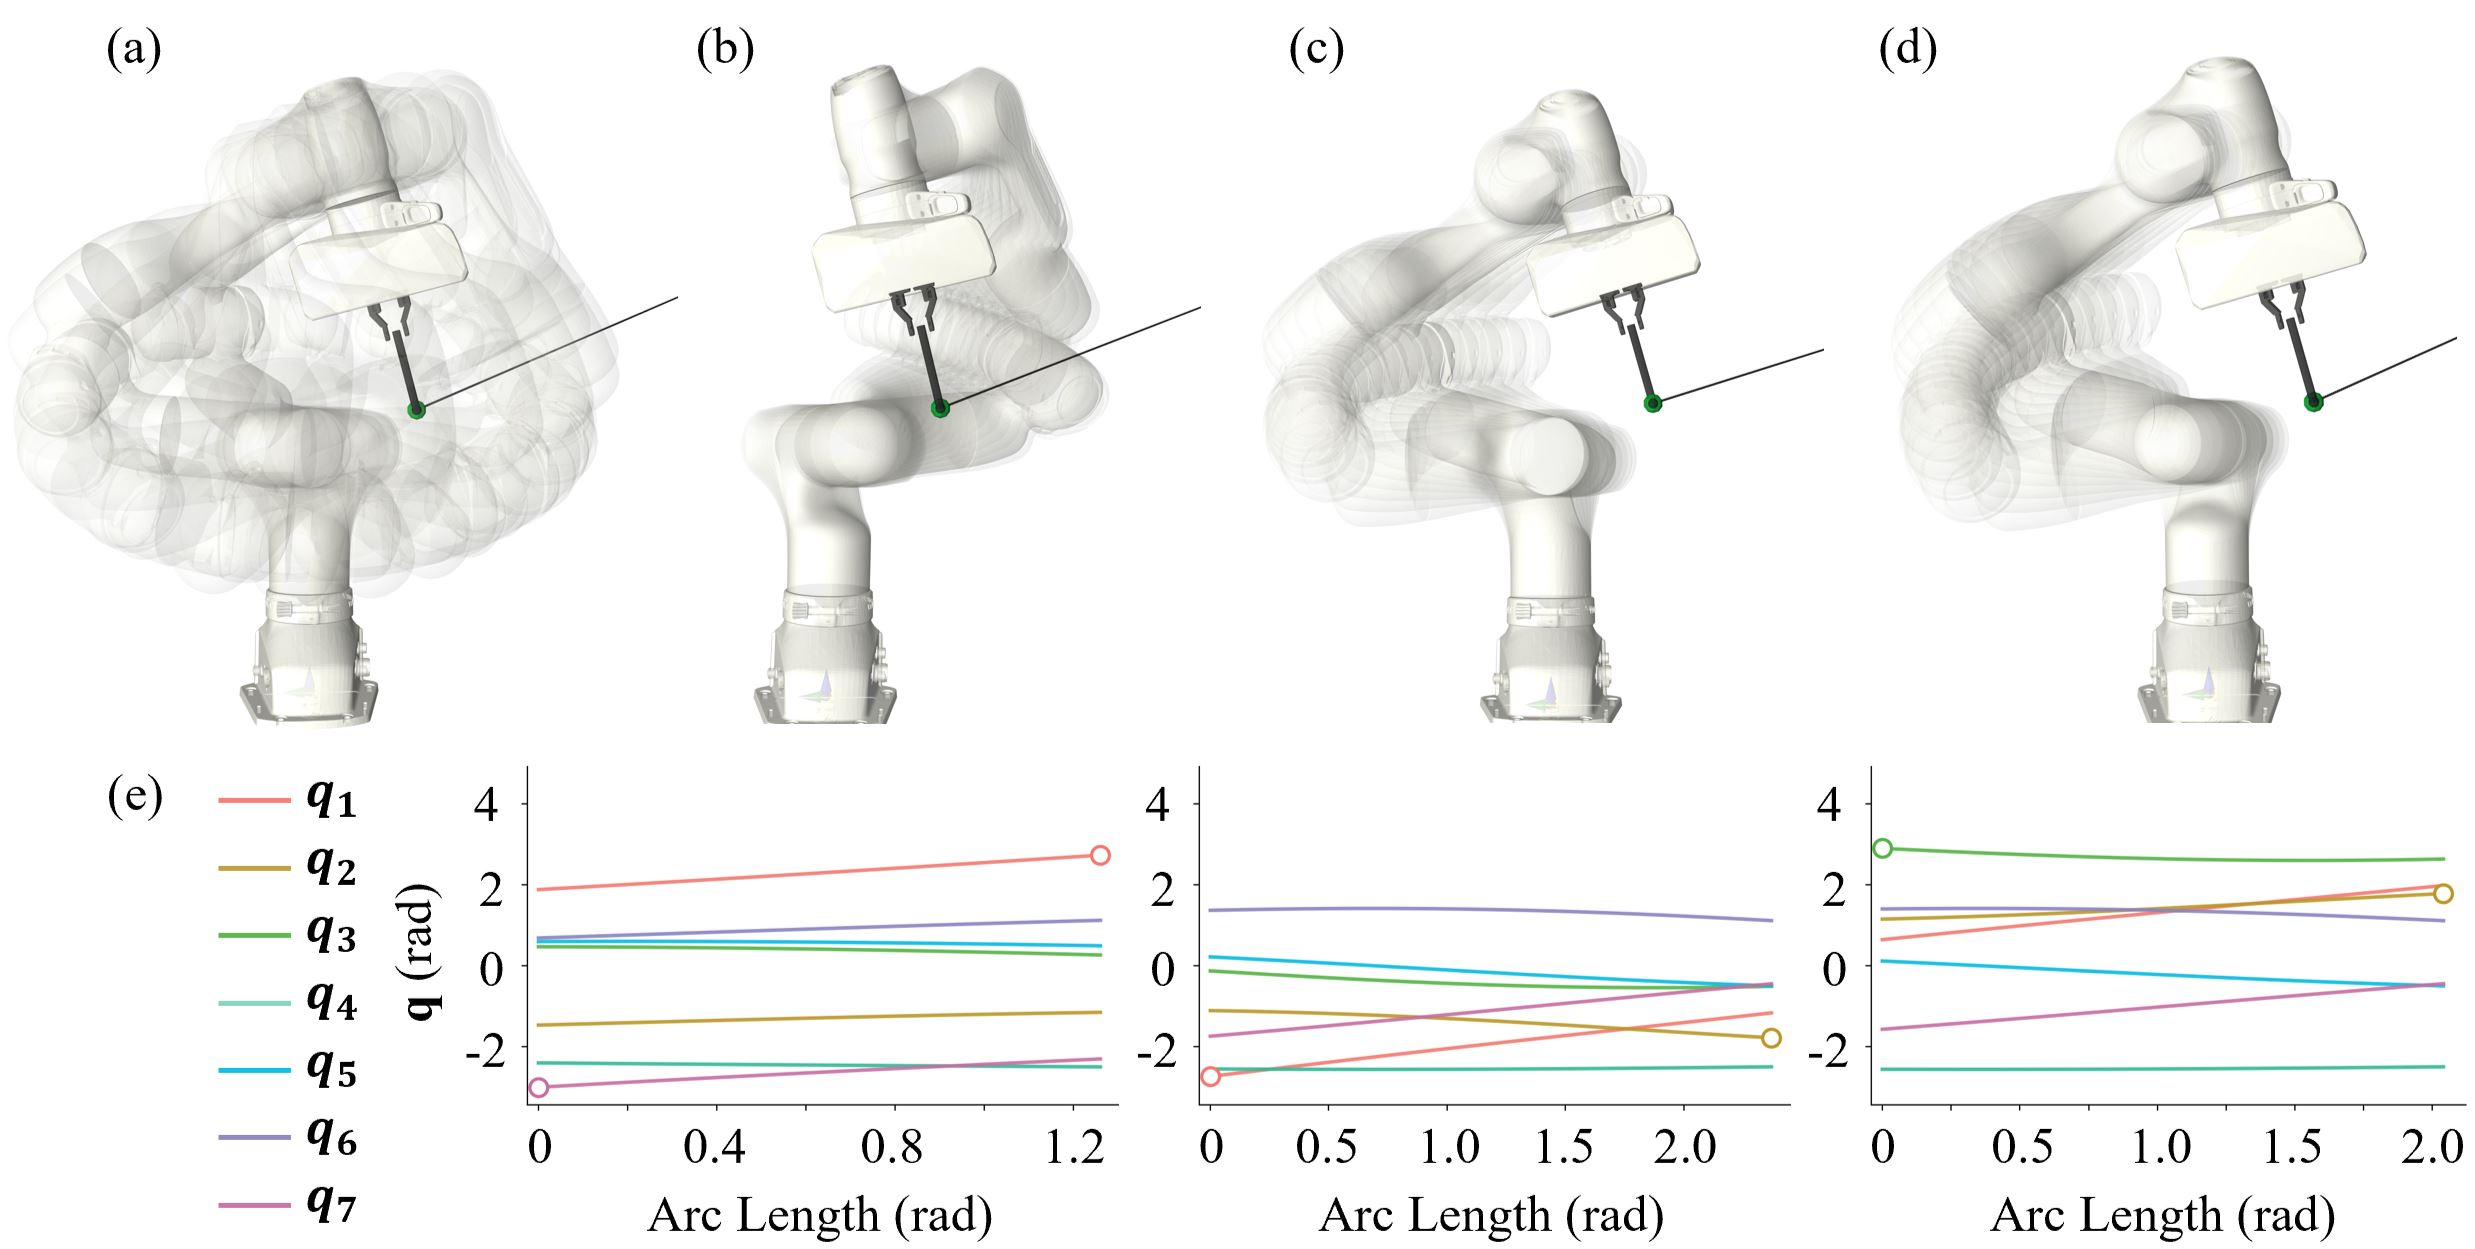
\includegraphics[width=\linewidth]{imgs/smm.JPG}
    \caption{Self-motion manifold for a fixed end-effector pose. (a) The continuous manifold without joint-limit constraints; (b)--(d) Configurations from the disconnected branches induced by the joint limits, sharing the same pose but differing sharply in joint space and reachable path length. (e) Joint trajectories of the three branches in b--d along the arc length, with circles marking the joint at its limit: branch~b bounded by $\mathbf{q}_{1}$ and $\mathbf{q}_{7}$, branch~c by $\mathbf{q}_{1}$, and $\mathbf{q}_{2}$ branch~d by $q_{2}$ and $\mathbf{q}_{3}$.}
    \label{smm}
\end{figure}

Therefore, this selection module aims to provide \new{the trajectory generation stage} with an initial joint configuration within a favorable branch. \new{Consequently, what the candidate layer must supply is coverage of the branches rather than precision of any single candidate, since every retained candidate is refined by damped least squares before use. For each task we query the pre-built IKSel table~\cite{yuan2026iksel} along $N_{\mathrm{dir}}$ tool directions sampled inside the orientation cone, rerank the retrieved entries by the full six-dimensional Jacobian metric, refine them under the cone constraint, remove duplicates, and reduce the survivors to $K$ candidates by farthest-point selection, appending the task-generating configuration as a fallback slot. What this layer is asked for is therefore diversity, not accuracy: a candidate that lands on a branch no other candidate reaches is worth more than one that sits marginally closer to the requested pose, and Fig.~\ref{fig:diversity} confirms that the achieved length saturates in the number of branches reached while being insensitive to how much each candidate is refined.}

\new{Which candidate to start from cannot be read off any instantaneous geometric quantity, because the consequence of the choice only becomes visible at the end of the stroke. The selector is therefore supervised by the outcome itself: every candidate of every training task is rolled out to termination under the analytic margin law of Eq.~(\ref{eq:margin-law}), and the resulting stroke lengths form the training targets. Because the resolution law is analytic, this supervision costs simulation time only --- no controller is trained, no annotation is made, and relabeling for a new manipulator or a new path family is a batch rollout.}

\new{Two properties of the scoring network match the structure of the decision. First, it is permutation-equivariant over the candidate set, encoding each candidate together with a mean-pooled context of the others, so that its score expresses a comparison within the task rather than an absolute prediction; training uses a listwise ranking objective on the within-task outcomes. Second, the score is conditioned on the task as a \emph{road table}: the path ahead of the start is sampled at fixed arc lengths, and the relative position, tangent and cone axis at each sample are concatenated into the input. The road table is what lets one selector serve every member of the path family of Section~III --- a straight ray, an arc, a serpentine seam and a rotating-axis path are all just different tables --- and Section~\ref{sec:setup} shows that a selector trained on straight and constant-curvature tasks alone transfers to families it has never seen. At deployment the choice costs one table query, one forward pass and one refinement; no candidate is rolled out.}

% \subsection{RL-based Null-Space Controller}
\subsection{Task-Constrained Joint Trajectory Generation}
\label{sec:traj}
\new{What this stage produces is a joint trajectory, not a stream of commanded
joint velocities: the velocities appear only as the increments used to construct
it, and nothing in the pipeline is closed on a measurement. Posing the stage
directly as a trajectory optimization is awkward, because the quantity to be
maximized is the length at which the trajectory ends, so neither the horizon nor
the number of decision variables is known before the problem is solved. Fixing a
horizon in advance either truncates the answer or spends variables on a stroke
that has already terminated.}

\new{We therefore generate the trajectory incrementally. At each increment the
end-effector is advanced along the prescribed path by a fixed arc length, and the
remaining freedom is used to choose among the joint displacements that realize
that advance. Working incrementally is also what keeps the tool on the path: the
position constraint of Eq.~\eqref{eq:pos_constraint} is imposed at every increment rather than spread
over a whole horizon, so the deviation never accumulates beyond the tolerance.
The redundancy at each increment is resolved in the null space of the position
Jacobian, following the decomposition of Eq.~\eqref{eq:nullspace}, and the only
design choice left is the null-space command $\mathbf{u}$.}

\new{The classical choice takes $\mathbf{u}$ from gradient ascent on the
weighted objective of Eq.~\eqref{eq:secondary}, which is evaluated entirely at
the current configuration. This is enough to steer away from a limit that is
about to be violated, but it cannot arrange the configuration now so that a
limit is not approached tens of increments later: the joint that eventually
terminates the stroke is usually not the joint the instantaneous objective is
pushing on, and the weights that trade the three terms against each other are
fixed for the whole stroke. The consequence is a stroke that ends well before
the path leaves the reachable workspace, which is the gap
Fig.~\ref{fig:pwgap} measures.}

\new{We therefore replace what the command reads, not the feedback form: the
secondary command is taken from the analytic margin law of
Eq.~(\ref{eq:margin-law}). At each increment the $2^{m}$ vertices of the
command box are scored by the margin field $\Phi_{\mathrm{m}}$ evaluated one
held command ahead --- the finite-rate form of the law --- and the maximizer
is executed. Reading a soft \emph{minimum} of all margins is what
distinguishes this from the weighted sum of Eq.~\eqref{eq:secondary}: the
field always pulls on whichever constraint is currently the closest exit, so
the balance among the competing constraints is re-chosen at every increment
rather than fixed by one set of weights, and reading the field by sign keeps
the command at full authority even where the margins are locally flat. On the
curved members of the path family the task term additionally carries a lateral
feedback that holds the tool inside the tolerance tube of
Eq.~\eqref{eq:pos_constraint}; it is inert on straight rays.}

Every resolution law in this paper outputs an $m$-dimensional command $\mathbf{a}\in[-1,1]^{m}$ \new{(written for $m=4$ below; Cobotta uses the same construction with $m=3$)} whose entries are coordinates in a task-aligned null-space basis $\mathbf{B}(\mathbf{q})\in\mathbb{R}^{7\times 4}$. The basis is constructed by Gram--Schmidt\new{ within the exact null space of the position Jacobian, identified by a double-precision SVD so that the null-space command cannot leak into the task motion}: the three projected gradients of the redundancy objectives in Eq.~\eqref{eq:secondary} are orthonormalized first, and the remaining one-dimensional orthogonal complement within the $4$-dimensional null space is appended to complete the basis. The resulting command $\dot{\mathbf{q}}_{\mathrm{null}}=\mathbf{B}(\mathbf{q})\,(a_{\max}\mathbf{a})$ is added to the same task term for every law in Eq.~\eqref{eq:nullspace}, so that all of them \new{share one parameterization and are interchangeable at any increment}.

\new{\paragraph*{Learned baseline policies} The experiments compare the
deployed law against policies trained with Proximal Policy Optimization (PPO)
under identical conditions, over the continuous box and over its $2^{m}$
vertices with a categorical head. Their observation exposes the quantities
needed to resolve the redundancy:}
\begin{equation}
\label{eq:obs}
\mathbf{o}_{t}=\big[\,\bar{\mathbf{q}};\ \bar{\mathbf{q}}^{\odot 2};\ \mathbf{d};\ \mathbf{n};\ \mathbf{z}(\mathbf{q});\ \mathbf{z}(\mathbf{q})^{\top}\mathbf{n};\ \mathbf{z}(\mathbf{q})\times\mathbf{n};\ \mathbf{a}_{t-1}\,\big],
\end{equation}
where $\bar{\mathbf{q}}$ is the joint configuration normalized to $[-1,1]$, whose element-wise square $\bar{\mathbf{q}}^{\odot 2}$ makes the proximity to either limit directly visible, and the tool-axis terms encode the orientation error relative to the cone; the end-effector position is excluded, as the deviation from the path is already held inside the tolerance by the task term. \new{Their reward is purely progress-based,}
\begin{equation}
\label{eq:reward}
r_{t} = w_{p}\,\mathrm{clip}\!\left(\frac{(\mathbf{p}_{t+1}-\mathbf{p}_{t})^{\top}\mathbf{d}}{v\,\Delta t},\,0,\,1\right)\in[0,\,w_{p}],
\end{equation}
with $w_{p}=1$ and no terminal penalty, \new{so the return approximates the
survival time and the trained policy pursues exactly the objective of
Eq.~(\ref{eq:value})}. \new{A supervised variant of the vertex policy
additionally hands the increment to the classical law inside a thin boundary
shell, entered when the normalized joint-limit distance}
\begin{equation}
\label{eq:rho}
\rho(\mathbf{q}) = \max_{i}\,\frac{|q_{i}-q_{\mathrm{mid},i}|}{(q_{\max,i}-q_{\min,i})/2}\in[0,1]
\end{equation}
\new{exceeds a threshold $\tau_{\mathrm{enter}}$ and left below
$\tau_{\mathrm{exit}}<\tau_{\mathrm{enter}}$ (hysteresis); because all laws
share the basis and the task term, the end-effector increment is unchanged at
a switch. Settings and sweeps are reported in Appendix~\ref{app:sweeps}.}

\subsection{\new{Where Learning Has Resolution}}
\label{sec:division}
\new{The two stages divide the work by the magnitude of the differences each
must discriminate, and both magnitudes are measured quantities. Across the
candidates of one task, the achievable strokes under the same resolution law
spread by hundreds of millimeters (Section~\ref{sec:setup}); a value network
regressing these outcomes from the start state reaches $R^{2}$ above $0.9$,
so the between-candidate signal is comfortably above what a learned score
resolves. Within one configuration, by contrast, the $2^{m}$ vertices differ
in one-step margin by $5\times10^{-3}$ to $2\times10^{-2}$ in normalized
units --- two orders of magnitude smaller --- and exactly this quantity is
what the analytic gradient of Eq.~(\ref{eq:margin-law}) supplies in closed
form. Learning is therefore placed where its resolution exceeds the signal
(the selection layer), and the closed form where the signal sits below that
resolution (the control layer). Section~\ref{sec:probes} verifies the
division from both sides with controlled probes at each layer.}

%%%%%%%%%%%%%%%%%%%%%%%%%%%%%%%%%%%%%%%%%%%%%%%%%%%%%%%%%%%%%%%%%%%%%%%%%
\section{Experiments and Analysis}
\label{sec:setup}
\new{All experiments were conducted using the \textit{One} robotic
system\footnote{https://github.com/wanweiwei07/one} on three manipulators: the
7-DoF xArm7, the 7-DoF Franka Research 3 (FR3), and the 6-DoF Cobotta, each with
a pen-shaped tool attached to the end-effector. The three differ in reach, in
joint ranges and, for Cobotta, in the dimension of the null space left by the
3-DoF position task, so they test whether the framework depends on a particular
amount of redundancy rather than on the structure of the problem. The same
candidate layer, selector architecture and resolution law are used on all
three --- the margin law of Eq.~(\ref{eq:margin-law}) has no per-manipulator
gains at all; only the kinematic model and the settings of
Table~\ref{tab:hyper} change.} The evaluation set \new{for each manipulator} comprises $10{,}000$ tasks, each specified by a starting position $\mathbf{p}_0$, a desired line direction $\mathbf{d}$, and a task-plane normal $\mathbf{n}$, sampled \new{within that manipulator's own work range, so the three sets are not in correspondence and only the realized fraction is comparable across them}. \new{The evaluation tasks are disjoint from those used to train the selector and the policy.} 

\new{Unless otherwise specified, experiments use the default setting: (1) a candidate pool of $K$ configurations retrieved from the IKSel table along $N_{\mathrm{dir}}$ directions inside the orientation cone, with the task-generating configuration as a fallback slot; (2) a road-table-conditioned selector that picks one candidate, followed by a single damped-least-squares refinement and no deployment-time rollout; (3) the analytic margin law in its finite-rate (one-step) form with temperature $\tau_{\mathrm{m}}=0.1$. Baseline settings --- the classical weights $k_{\mu},k_{\mathrm{jl}},k_{\theta}$ and the hybrid thresholds $\tau_{\mathrm{enter}},\tau_{\mathrm{exit}}$ of the supervised PPO variant --- are reported per manipulator in Table~\ref{tab:hyper}.}

\new{A stroke has to pass through every point of the prescribed path up to the point where it stops, so the first point at which no admissible configuration exists bounds the achievable length from above. We march along each task's own path and, at every sample, search for a configuration that places the tool within the position tolerance of Eq.~\eqref{eq:pos_constraint} and keeps the tool axis inside the cone of Eq.~\eqref{eq:ori_constraint} without violating joint limits or self-collision. The arc length of the first sample at which this search fails is the \emph{pointwise-reachable length} $\ell^{\mathrm{pw}}$, and we report the achieved length as the fraction $\mathcal{L}/\ell^{\mathrm{pw}}$ of it that a single continuous stroke realizes. Unlike a best-of-$K$ reference, this quantity involves no resolution law; because the per-sample feasibility test is a finite search, its status as an upper bound is checked rather than assumed --- Table~\ref{tab:bound} verifies that no executed stroke exceeds it and that it is stable under a doubled search budget.}

\new{We group the evaluation set by stroke length rather than by difficulty, using the terciles of $\ell^{\mathrm{pw}}$ within each manipulator: long-, medium- and short-stroke. Because the boundaries are defined per manipulator, the realized fraction is comparable across methods on one manipulator, while absolute path lengths are not comparable across manipulators. Grouping by stroke length also avoids reading a geometric property of the task as a statement about how hard it is.}


% skeleton: per-manipulator hyper-parameters referenced by the setup paragraph
\begin{table}[!htbp]
\centering
\color{red}
\caption{\new{Per-manipulator settings held fixed across all experiments.}}
\label{tab:hyper}
\begin{tabular}{lccc}
\toprule
& xArm7 & Franka Research 3 & Cobotta \\
\midrule
DoF                                          & 7 & 7 & 6 \\
Null-space dimension                         & 4 & 4 & 3 \\
Cone half-angle $\theta_{\max}$              & $30^{\circ}$ & $30^{\circ}$ & $30^{\circ}$ \\
Candidates $K$ / directions $N_{\mathrm{dir}}$ & -- & -- & -- \\
Margin-law temperature $\tau_{\mathrm{m}}$    & 0.1 & 0.1 & 0.1 \\
$(\tau_{\mathrm{enter}},\tau_{\mathrm{exit}})$ (baseline) & (0.98, 0.94) & (0.98, 0.94) & (0.98, 0.94) \\
$(k_{\mu},k_{\mathrm{jl}},k_{\theta})$ (classical law) & (0.8, 0.4, 0.2) & (0.8, 0.4, 0.2) & (0.8, 0.4, 0.2) \\
Evaluation tasks                              & -- & -- & -- \\
\bottomrule
\end{tabular}
\end{table}

\subsection{\new{Evaluation Protocol}}
\new{Every number below is a fraction of $\ell^{\mathrm{pw}}$, so the protocol is
only as trustworthy as that quantity. Two properties have to hold. First,
$\ell^{\mathrm{pw}}$ must not be exceeded; otherwise it is a reference, not a
bound. Second, it must not depend on how hard the feasibility test searches,
since a bound that grows with the search budget is an artifact of the solver.
Table~\ref{tab:bound} reports both: the fraction of tasks on which any executed
stroke exceeds the bound, and how the bound moves when the search budget is
doubled. We also report the same two quantities for two references that are
easier to compute and that fail the first test --- a voxelized reachability
chord, and the best-of-$K$ reference used in our earlier
version~\cite{yuan2026extreme} --- since their failure is what motivates the
per-task march.}

\new{Statistics are reported the same way throughout. Comparisons between
methods are paired per task and summarized by the mean, the median and the
$10$th--$90$th percentile range of the realized fraction; differences carry
paired bootstrap $95\%$ confidence intervals over tasks, together with the
fraction of tasks on which one method exceeds the other. For learned methods,
two independent training runs of one configuration set the noise floor, and
differences within that spread are reported as indistinguishable rather than
ranked.}

% skeleton: validity and convergence of the denominator
\begin{table}[!htbp]
\centering
\color{red}
\caption{\new{Validity and convergence of the reported denominator. A reference
is usable only if no executed stroke exceeds it and if it is stable under a
larger feasibility-search budget.}}
\label{tab:bound}
\begin{threeparttable}
\begin{tabular}{lccc}
\toprule
Reference & \shortstack{Exceeded on\\(\% of tasks)} & \shortstack{Worst\\ratio} & \shortstack{Change on\\budget $\times 2$} \\
\midrule
Best-of-$K$ rollouts~\cite{yuan2026extreme} & -- & -- & n/a \\
Voxelized reachability chord             & -- & -- & n/a \\
\textbf{$\ell^{\mathrm{pw}}$ (ours)}     & -- & -- & -- \\
\bottomrule
\end{tabular}
\begin{tablenotes}
    \item[Note 1] \new{The first two rows are computed for comparison only and
    are not used to report any result in this paper.}
    \item[Note 2] \new{Budget is the number of tool directions sampled inside the
    cone and the number of warm starts per direction.}
\end{tablenotes}
\end{threeparttable}
\end{table}

\subsection{\new{Controller Ladder and End-to-End Comparison}}

\new{Because no prior method optimizes the feasible extent itself, the
comparisons are not drawn from adjacent papers but constructed as a ladder of
solution strategies for the exit-time problem of Section~\ref{sec:hjb}, each
rung answering one question. From below, the ladder establishes what the
deployed law adds: no null-space motion ($\mathbf{a}=\mathbf{0}$) prices the
redundancy itself; the classical law prices the hand-weighted instantaneous
surrogate; the analytic margin law of Eq.~(\ref{eq:margin-law}) then differs
from the classical rung only in the two substitutions of
Section~\ref{sec:relation}, so its margin over that rung measures exactly
what reading the right field by sign is worth. From above, the ladder
establishes what the deployed law leaves unclaimed: receding-horizon
optimizers (cross-entropy search and beam search over vertex sequences)
maximize the \emph{same} margin objective over $H$ held commands with the
environment itself as the model, so any headroom above the one-step law must
appear in their rungs. Learned policies --- continuous PPO, vertex PPO, and
the supervised vertex variant of Section~\ref{sec:traj} --- are included as
baselines under identical conditions. All rungs share the task term, the
constraint set and the initial configuration, so the comparison isolates the
secondary command; the optimization-based rungs are evaluated on a
$1024$-task subset and all others on the full set.}

\new{Table~\ref{tab:mainresult} reports the ladder on the main protocol, and
three views unpack it. Table~\ref{tab:horizon} sweeps the optimizer horizon
$H$: the analytic law needs no search, so the operative question is how much
of the exactly-optimized performance it already attains, and at what fraction
of the per-increment cost. Table~\ref{tab:termcause} reports what ends each
stroke; a longer mean is evidence about the mechanism when it comes with
terminations converted away from the constraint the lower rungs die on.
Fig.~\ref{fig:survival} shows the survival function
$S(x)=\Pr[\mathcal{L}/\ell^{\mathrm{pw}}\ge x]$, which makes visible whether
a method shifts the whole distribution or only stretches its tail. The
deviation from the prescribed path is bounded by $\epsilon_{\mathrm{pos}}$ by
construction, and its maximum over all strokes is reported as a note to
Table~\ref{tab:mainresult}; per-query computation appears in the last column
of Table~\ref{tab:ablate_seed}.}

% skeleton: the horizon ladder, C1 evidence
\begin{table}[!htbp]
\centering
\color{red}
\caption{\new{The analytic law against exact optimization of the same margin
objective over longer horizons, on a $1024$-task subset. What the table
establishes is a plateau: extending the horizon beyond one held command adds
performance within the task-level noise, and the one-gradient law sits on the
plateau at a small fraction of the per-increment cost.}}
\label{tab:horizon}
\begin{tabular}{lccc}
\toprule
Controller & \shortstack{Horizon\\(held commands)} & Realized (\%) & \shortstack{Per-step\\compute (ms)} \\
\midrule
Margin law, gradient form (Eq.~\ref{eq:margin-law}) & 0 & -- & -- \\
Margin law, one-step form (ours)  & 1 & -- & -- \\
Receding CEM ($H=4$)   & 4  & -- & -- \\
Receding CEM ($H=8$)   & 8  & -- & -- \\
Beam search ($H=8$)    & 8  & -- & -- \\
Receding CEM ($H=16$)  & 16 & -- & -- \\
\bottomrule
\end{tabular}
\end{table}

% skeleton: termination causes as a main result
\begin{table}[!htbp]
\centering
\color{red}
\caption{\new{What ends the stroke (\% of tasks). The mechanism claim is
here: a method that reaches farther must show which termination it defers,
not only a larger mean.}}
\label{tab:termcause}
\begin{tabular}{lccccc}
\toprule
Controller & Joint & Cone & Collision & Tracking & Cap \\
\midrule
No null-space          & -- & -- & -- & -- & -- \\
Classical law          & -- & -- & -- & -- & -- \\
Continuous PPO         & -- & -- & -- & -- & -- \\
Vertex PPO             & -- & -- & -- & -- & -- \\
Receding CEM ($H=16$)  & -- & -- & -- & -- & -- \\
\textbf{Margin law (ours)} & -- & -- & -- & -- & -- \\
\bottomrule
\end{tabular}
\end{table}

% skeleton: survival curves, the exit-time view of the same data
\begin{figure}[!htbp]
    \centering
\color{red}
    \fbox{\parbox[c][4.0cm][c]{0.92\linewidth}{\centering
    \new{[Placeholder] Left: survival function $S(x)=\Pr[\mathcal{L}/\ell^{\mathrm{pw}}\ge x]$
    per rung of the ladder. A rightward shift of the whole curve, rather than
    a heavier tail, is what distinguishes a systematic gain from a few
    rescued outliers. Right: paired gain of the margin law over the
    classical law against three difficulty coordinates of the task ---
    initial joint-limit margin, initial $\sigma_{\min}(\mathbf{J})$, initial
    cone margin --- in deciles.}}}
    \caption{\new{Distributional view of the main comparison. Left: the
    exit-time formulation makes the survival function, not the mean alone,
    the natural summary. Right: where the gain concentrates; the exit-time
    view predicts it grows as the start approaches a future feasibility
    bottleneck.}}
    \label{fig:survival}
\end{figure}

\new{The full system --- the selector of Section~\ref{sec:select} feeding the
analytic margin law --- appears as the last row of
Table~\ref{tab:mainresult}. Fig.~\ref{fig:attribution}
then separates the two stages: starting from the first feasible candidate under
the classical law, we replace only the initial configuration, then only the
trajectory generation, and read the increment attributable to each. The
decomposition matters because the two stages are not interchangeable, the choice
of branch is made once and cannot be revised during the stroke, whereas the
trajectory stage acts at every increment but only within the branch it was
given.}


% skeleton: attribution of the realized fraction to the two stages
\begin{figure}[!htbp]
    \centering
\color{red}
    \fbox{\parbox[c][4.2cm][c]{0.92\linewidth}{\centering
    \new{[Placeholder] Stacked attribution: starting from the first feasible
    candidate under the classical null-space law, the fraction added by
    replacing the candidate (stage one) and the fraction added by replacing the
    trajectory stage (stage two), per stroke bucket and per manipulator.}}}
    \caption{\new{How much of the pointwise-reachable length each stage
    realizes. The gap that remains at the top is the part no combination of the
    two stages recovers.}}
    \label{fig:attribution}
\end{figure}
\begin{table*}[!htbp]
\centering
\setlength{\tabcolsep}{5pt}
\caption{Realized fraction of the pointwise-reachable length across three manipulators and stroke-length
buckets. Each cell reports the achieved Cartesian path length (m) and the fraction of the
pointwise-reachable length realized by a single continuous stroke (\%); no stroke exceeds
$100\%$, a property verified in Table~\ref{tab:bound} rather than assumed. Best results in \textbf{bold}.}
\label{tab:mainresult}
\begin{threeparttable}
\begin{tabular}{l cccc cccc cccc}
\toprule
& \multicolumn{4}{c}{xArm7} & \multicolumn{4}{c}{Franka Research 3} & \multicolumn{4}{c}{Cobotta} \\
\cmidrule(lr){2-5}\cmidrule(lr){6-9}\cmidrule(lr){10-13}
Method & All & L & M & S & All & L & M & S & All & L & M & S \\
\midrule
No null-space ($\mathbf{a}=\mathbf{0}$) & 0 / 0 & 0 / 0 & 0 / 0 & 0 / 0 & 0 / 0 & 0 / 0 & 0 / 0 & 0 / 0 & 0 / 0 & 0 / 0 & 0 / 0 & 0 / 0 \\
Classical null-space law        & 0 / 0 & 0 / 0 & 0 / 0 & 0 / 0 & 0 / 0 & 0 / 0 & 0 / 0 & 0 / 0 & 0 / 0 & 0 / 0 & 0 / 0 & 0 / 0 \\
Continuous PPO                  & 0 / 0 & 0 / 0 & 0 / 0 & 0 / 0 & 0 / 0 & 0 / 0 & 0 / 0 & 0 / 0 & 0 / 0 & 0 / 0 & 0 / 0 & 0 / 0 \\
Vertex PPO                      & 0 / 0 & 0 / 0 & 0 / 0 & 0 / 0 & 0 / 0 & 0 / 0 & 0 / 0 & 0 / 0 & 0 / 0 & 0 / 0 & 0 / 0 & 0 / 0 \\
Vertex PPO + supervisor         & 0 / 0 & 0 / 0 & 0 / 0 & 0 / 0 & 0 / 0 & 0 / 0 & 0 / 0 & 0 / 0 & 0 / 0 & 0 / 0 & 0 / 0 & 0 / 0 \\
Receding CEM ($H=16$)           & 0 / 0 & 0 / 0 & 0 / 0 & 0 / 0 & 0 / 0 & 0 / 0 & 0 / 0 & 0 / 0 & 0 / 0 & 0 / 0 & 0 / 0 & 0 / 0 \\
Margin law (ours)               & 0 / 0 & 0 / 0 & 0 / 0 & 0 / 0 & 0 / 0 & 0 / 0 & 0 / 0 & 0 / 0 & 0 / 0 & 0 / 0 & 0 / 0 & 0 / 0 \\
\textbf{Full system (selector + margin law, ours)} & \textbf{0 / 0} & \textbf{0 / 0} & \textbf{0 / 0} & \textbf{0 / 0}
                                & \textbf{0 / 0} & \textbf{0 / 0} & \textbf{0 / 0} & \textbf{0 / 0}
                                & \textbf{0 / 0} & \textbf{0 / 0} & \textbf{0 / 0} & \textbf{0 / 0} \\
\bottomrule
\end{tabular}
\end{threeparttable}
\begin{tablenotes}
    \item ${}^{\text{Note 1~}}$ Each cell is formatted as path length (m) / realized fraction (\%). \new{All controller rows share the same per-task initial configuration; the full system additionally applies the learned selector. The CEM row is evaluated on a $1024$-task subset.}
    \item ${}^{\text{Note 2~}}$ L / M / S denote long-, medium-, and short-stroke buckets, defined per manipulator by terciles of the pointwise-reachable length, so that the bucket boundaries adapt to each manipulator's work range rather than being fixed at absolute thresholds. Consequently, the realized fraction is comparable across methods within one manipulator, whereas absolute path lengths are not comparable across manipulators.
    \item ${}^{\text{Note 3~}}$ Cobotta is a 6-DoF manipulator. Under the 3-DoF position task the null space is correspondingly reduced, and the same null-space parameterization is applied with a reduced action basis.
\end{tablenotes}
\end{table*}

\subsection{Ablation Study}

\subsubsection{\new{Branch Coverage of the Candidate Pool}}
\label{sec:branch}
\new{The premise of the whole first stage is that the candidates differ in which
branch of the self-motion manifold they occupy, since otherwise choosing among
them would be a continuous adjustment of the kind the trajectory stage already
performs. We test this directly. Two candidates of the same task are assigned to
the same branch when one can be carried into the other by a continuous motion
that holds the tool position fixed, keeps the tool axis inside the cone, and
respects the joint limits; the assignment is computed by connectivity in that
constraint set. Table~\ref{tab:branch} reports how many branches a pool of $K$
candidates reaches, how often the selected candidate lies on a different branch
from the first feasible one, and how much of the achieved length is associated
with the branch rather than with the position within it.}

% skeleton: branch coverage of the candidate pool
\begin{table}[!htbp]
\centering
\color{red}
\caption{\new{Branch coverage of the candidate pool, and the share of achieved
task-space length associated with the branch rather than with the configuration
chosen inside it.}}
\label{tab:branch}
\begin{tabular}{lccc}
\toprule
& xArm7 & FR3 & Cobotta \\
\midrule
Branches reached per task (median)          & -- & -- & -- \\
Selected candidate on a different branch (\%) & -- & -- & -- \\
Spread within a branch / spread across branches & -- & -- & -- \\
Share of achieved length attributable to the branch (\%) & -- & -- & -- \\
\bottomrule
\end{tabular}
\end{table}

\subsubsection{Supervision Signal}
\label{sec:ablate_seed}
\new{With the branches established, the question is what the choice among them
can be based on. We compare the outcome-supervised selector against criteria
that are computable at the start of the stroke: the manipulability-maximizing
and joint-limit-centering initializations, both obtained by null-space ascent from the
task-generating configuration and therefore confined to its branch, and a
predictor trained on those same local quantities instead of on realized
returns.}
\new{Table~\ref{tab:ablate_seed} fixes the trajectory stage and varies only where the stroke starts, so every difference is attributable to the initial configuration. The two heuristic initializations ascend the null-space gradient from the task-generating configuration; because that ascent stays inside the null space it cannot cross a joint limit, and both therefore remain on the branch they started from. Fig.~\ref{fig:diversity} then separates the two properties of the candidate layer, the number of branches it covers and the accuracy of each candidate, and shows which of them the result depends on.}
% skeleton: candidate layer and selector ablation
\begin{table}[!htbp]
\centering
\color{red}
\caption{\new{Initial configuration selection under a fixed trajectory stage.
\emph{Capture} is the share of the gap between a random feasible candidate and
the best candidate in the same pool that the selector recovers.}}
\label{tab:ablate_seed}
\begin{threeparttable}
\begin{tabular}{lcccc}
\toprule
Initial configuration & \shortstack{Length\\(m)} & \shortstack{Realized\\(\%)} & \shortstack{Capture\\(\%)} & \shortstack{Time\\(ms)} \\
\midrule
Task-generating configuration & -- & -- & -- & -- \\
Manipulability-maximizing initialization & -- & -- & -- & -- \\
Joint-limit-centering initialization     & -- & -- & -- & -- \\
Random feasible candidate      & -- & -- & \phantom{--}0 & -- \\
First feasible candidate       & -- & -- & -- & -- \\
\textbf{Selector (ours)}       & -- & -- & -- & -- \\
\midrule
Within-pool oracle             & -- & -- & 100 & -- \\
\bottomrule
\end{tabular}
\begin{tablenotes}
    \item[Note 1] \new{All rows share the same motion stage, so the differences
    are attributable to the initial configuration alone.}
    \item[Note 2] \new{The two heuristic initializations ascend the null-space gradient
    from the task-generating configuration and therefore cannot leave its branch;
    the candidate pool is what makes other branches reachable at all.}
\end{tablenotes}
\end{threeparttable}
\end{table}

\begin{figure}[!htbp]
    \centering
    \color{red}
    \fbox{\parbox[c][3.8cm][c]{0.92\linewidth}{\centering
    \new{[Placeholder] Realized fraction against the number of \emph{branches}
    the pool reaches, overlaid with the same data plotted against the number of
    candidates, showing that the former is what the curve is a function of;
    an inset sweeps the refinement iterations per candidate at fixed $K$.}}}
    \caption{\new{What the candidate layer has to deliver is branch coverage:
    candidates added within a branch already reached do not help, and the
    result is flat in how much each candidate is refined.}}
    \label{fig:diversity}
\end{figure}

\subsubsection{\new{Path Conditioning and Out-of-Family Generalization}}
\label{sec:ood}
\new{The road table of Section~\ref{sec:select} is what makes the selector a
function of the task rather than of the start state alone, and its value is
measurable by ablation: an unconditioned twin --- identical architecture and
training, with the road table removed from the input --- can only rank
candidates by properties of the start. Both selectors are trained on
$20{,}000$ tasks drawn from the straight and constant-curvature families
alone, and evaluated on $10{,}000$ held-out tasks spanning all four families
of Section~III, so that the serpentine and rotating-axis families are
strictly outside the training distribution. Labels come from rollouts of the
analytic law; candidates come from the same layer on every family.
Table~\ref{tab:ood} reports, per family, the share of the gap between a
random feasible candidate and the best candidate that each selector captures,
the top-1 regret, and the within-task rank correlation, alongside the
task-generating configuration as the training-free reference.}

% selector generalization across path families (fill from runs/selector_ood/v1)
\begin{table}[!htbp]
\centering
\color{red}
\caption{\new{Selector generalization across path families. Trained on
straight and arc tasks only; serpentine and rotating-axis rows are
out-of-family. \emph{Capture} is the share of the random-to-oracle gap
recovered; $\rho_{s}$ is the mean within-task Spearman correlation.}}
\label{tab:ood}
\begin{tabular}{llcccc}
\toprule
Family & Split & Selector & Capture & Regret & $\rho_{s}$ \\
\midrule
Straight    & in     & conditioned   & -- & -- & -- \\
            &        & unconditioned & -- & -- & -- \\
Arc         & in     & conditioned   & -- & -- & -- \\
            &        & unconditioned & -- & -- & -- \\
Serpentine  & out    & conditioned   & -- & -- & -- \\
            &        & unconditioned & -- & -- & -- \\
Rotating axis & out  & conditioned   & -- & -- & -- \\
            &        & unconditioned & -- & -- & -- \\
\bottomrule
\end{tabular}
\end{table}

\subsubsection{Classical Null-Space Law Hyperparameters}
\new{The weights of Eq.~\eqref{eq:secondary} were selected by a $39$-setting sweep, reported in Appendix~\ref{app:sweeps}: single objectives are uniformly weak, any mixed combination surpasses them, and no combination improves meaningfully across the full evaluation set, so the tuned setting of Table~\ref{tab:hyper} is used throughout.}

\subsubsection{\new{Action-Space Structure}}
\new{The sweep also says something about the shape of the command, not only
its weighting. Expressed in the same basis the policy acts in, the classical
command is an interior point of the admissible box: its median magnitude is
$0.14$ of the box half-width and it lies within $10\%$ of the boundary on $0.1\%$
of steps, because gradient ascent produces a command whose size is that of the
gradient. The learned policy sits at the opposite extreme, with median
magnitude $1.00$ and $89.2\%$ of steps on the boundary. Two checks show that the
magnitudes it can express are not what it is using. Projecting its command onto
the nearest vertex of the box --- replacing each coordinate by its sign ---
changes the realized length by $+0.004$ alone and $+0.005$ inside the hybrid,
both with bootstrap intervals spanning zero. And a policy whose action space
\emph{is} the $2^{4}$ vertices, trained from scratch with a categorical head,
exceeds it: $+0.088$ for the policy alone and $+0.042$ inside the hybrid, in
the ratio to the classical law and with paired intervals excluding zero
(Table~\ref{tab:action_space}). Proposition~\ref{prop:vertex} predicts no loss
in the continuous-time optimum, so the gain is attributable to the
parameterization being easier to optimize, not to a larger admissible set;
Fig.~\ref{fig:optdiag} shows the training-side evidence, the entropy of the
continuous policy pinned at its ceiling by tanh saturation while the
categorical policy converges normally. For this task the learned continuous
resolution therefore behaves as a discrete switching controller over the extreme
null-space directions: what it has learned is which extreme direction to take as
a function of configuration, not how far along that direction to push. This is
the switching structure that Section~\ref{sec:hjb} derives from the exit-time
formulation.
}

% skeleton: continuous against vertex-valued action spaces
\begin{table}[!htbp]
\centering
\color{red}
\caption{\new{The command box against its vertices. Projection (row two)
tests whether the magnitudes carry information; native vertex training (row
three) tests whether the restriction costs learned performance. Ratios are to
the classical law on identical tasks; differences are paired against row
one.}}
\label{tab:action_space}
\begin{tabular}{lcccc}
\toprule
Null-space command & \shortstack{Policy\\ratio} & \shortstack{Hybrid\\ratio}
& \shortstack{$\Delta$ policy\\{[}95\% CI{]}} & \shortstack{$\Delta$ hybrid\\{[}95\% CI{]}} \\
\midrule
Continuous in $[-1,1]^{4}$      & 1.295 & 1.398 & --- & --- \\
Projected onto nearest vertex   & 1.299 & 1.403 & $+0.004$ {\scriptsize$[\ni 0]$} & $+0.005$ {\scriptsize$[\ni 0]$} \\
Trained over the $2^{4}$ vertices & \textbf{1.383} & \textbf{1.440} & $+0.088$ {\scriptsize$[+0.057,+0.119]$} & $+0.042$ {\scriptsize$[+0.014,+0.070]$} \\
\bottomrule
\end{tabular}
\end{table}

% skeleton: optimization diagnostics of the two parameterizations
\begin{figure}[!htbp]
    \centering
\color{red}
    \fbox{\parbox[c][3.8cm][c]{0.92\linewidth}{\centering
    \new{[Placeholder] Two panels under identical training conditions.
    Left: policy entropy over training, the continuous policy pinned at its
    saturation ceiling against the categorical policy converging from
    $\log 16$. Right: saturation statistics of the continuous policy ---
    distribution of $|\mathbf{a}|$, of the pre-squash mean, and of the tanh
    slope at the executed action.}}}
    \caption{\new{Why the vertex parameterization trains better: the
    continuous policy must express vertices through a saturated squashing
    function, which attenuates its gradient; the categorical policy has no
    such bottleneck.}}
    \label{fig:optdiag}
\end{figure}


{\color{red}
\subsubsection{Resolution Probes at Both Layers}
\label{sec:probes}
The division of labor stated in Section~\ref{sec:division} rests on two
measured scales, and each is probed where it operates. At the selection
layer, a value network regressing the analytic-law outcome from the
$27$-dimensional start-state encoding reaches $R^{2}=0.91$ on held-out tasks
with a within-task ranking correlation of $0.92$: the between-candidate
signal, which spreads over hundreds of millimeters, is comfortably inside
what a learned score resolves, and this is the capacity the selector of
Section~\ref{sec:select} exploits. At the control layer, the corresponding
signal is the within-state spread of the one-step margins of the $2^{m}$
vertices, measured at $5\times10^{-3}$ to $2\times10^{-2}$ in normalized
units on the deployed law's own trajectories --- two orders of magnitude
below the selection-layer signal. Controlled probes confirm that this scale
separation, not any particular training choice, is what governs where
learning helps: supervised and value-based predictors trained at the control
layer on the same data rank the $2^{m}$ vertices no better than the analytic
gradient that is available for free, across the parameterizations summarized
in Appendix~\ref{app:sweeps}, while the identical machinery at the selection
layer learns its target well. The architecture therefore assigns each layer
the instrument whose resolution matches its signal: a learned score above,
a closed-form gradient below.
}




\subsubsection{\new{Cross-Arm Replication}}
\label{sec:crossarm}
{\color{red}
Everything above was measured on one arm; this subsection asks what
replicates when only the embodiment changes. The pipeline was ported to the
xArm7 and the Cobotta with every experimental setting shared --- the same
task speed, control period, command bound, cone, and, for the learned
baselines, the same reward and PPO configuration --- so the action space
follows the morphology alone: $2^{4}$ vertices for the 7-DoF arms, $2^{3}$
for the Cobotta, whose three objective gradients fill its null space exactly.
The deployed margin law requires nothing to port beyond the kinematic model:
its field, its temperature and its one-step form are morphology-independent
by construction, and its margin over each arm's classical law is reported in
the first data row of Table~\ref{tab:multiarm}.

The mechanism replicates alongside the numbers. On every arm the classical
law dies overwhelmingly on the cone ($81$--$85\%$), and the vertex-switching
resolutions --- analytic and learned baseline alike --- convert part of
those endings into longer strokes; the effective vertex-switching rate
spends most of the $20$\,Hz control budget on every arm ($16.3$, $16.7$ and
$13.7$\,Hz for the baseline policies). The strategy is also one and the
same, made comparable by the shared basis semantics: on all three arms the
cone coordinate is pushed positive throughout the stroke and increasingly so
($+0.60\!\to\!+0.82$, $+0.72\!\to\!+0.92$, $+0.71\!\to\!+0.84$ from the
first to the last third), the manipulability coordinate is near-neutral
early and strongly positive late, the centering coordinate starts positive
and decays, and the orthogonal complement of the 7-DoF arms carries no
preference at all. This is one strategy instantiated three times --- bank
joint-limit margin while the stroke is young, then spend it defending the
quantities whose exhaustion ends strokes --- and it is the strategy the
margin field of Eq.~(\ref{eq:margin-field}) encodes explicitly.

The commonality extends to the weights. The two 7-DoF arms share the
$31$-dimensional observation layout, so the FR3-trained policy can be
executed on the xArm7 unchanged: zero-shot it reaches $1.337$ (policy) and
$1.382$ (hybrid) against the xArm7's classical law, retaining about $80\%$
of the natively trained gain ($1.410$/$1.440$) across different link
lengths, joint limits and collision geometry. In the normalized coordinates
of the observation, much of what the policy learned is not specific to the
arm it was trained on. What does scale with the embodiment is the size of
the gain: the Cobotta, with no spare null-space direction and tight joint
ranges, gains least, uses the centering coordinate sparingly (net $+0.10$
against $+0.72$ and $+0.55$), and offers the supervisor a third as many
takeover occasions.

% cross-arm summary, mechanism protocol
\begin{table}[!htbp]
\centering
\color{red}
\caption{\new{Cross-arm replication under the mechanism protocol (ratio to
each arm's classical law, $2048$ straight tasks per arm,
$\tau=(0.98,0.94)$).}}
\label{tab:multiarm}
\begin{tabular}{lccc}
\toprule
& FR3 & xArm7 & Cobotta \\
\midrule
Null-space dimension $m$ (vertices)   & 4 (16) & 4 (16) & 3 (8) \\
\textbf{Margin law / classical (ours)} & -- & -- & -- \\
Vertex policy / classical             & 1.399 & 1.410 & 1.256 \\
Hybrid / classical                    & 1.435 & 1.440 & 1.270 \\
Classical cone terminations (\%)      & 81.4 & 84.6 & 82.6 \\
Policy cone terminations (\%)         & 58.3 & 63.1 & 65.9 \\
Switching rate (Hz, of 20)            & 16.3 & 16.7 & 13.7 \\
FR3 policy zero-shot, hybrid          & ---  & 1.382 & n/a \\
\bottomrule
\end{tabular}
\end{table}
}

\subsubsection{\new{Executability of Vertex-Switching Strokes}}
\new{The deployed law switches among extreme null-space directions, so the
generated joint trajectory changes its null-space component discontinuously
at increments where the selected orthant changes. Two properties keep this
executable. Structurally, a switch alters only the null-space component of
the increment, so the end-effector motion is unaffected and the joint-space
discontinuity is bounded by $a_{\max}$. Quantitatively, we time-parameterize
the generated trajectories with a standard
method~\cite{pham2018toppra,berscheid2021ruckig} and report the resulting
velocity and acceleration profiles against the manufacturer limits in
Table~\ref{tab:continuity}, together with the profiles at the switching
increments in particular.}

% skeleton: executability of the generated trajectory
\begin{table}[!htbp]
\centering
\color{red}
\caption{\new{Executability after time parameterization. Reported over all
evaluation strokes and, separately, over the increments at which the resolution
switches.}}
\label{tab:continuity}
\begin{tabular}{lccc}
\toprule
& xArm7 & FR3 & Cobotta \\
\midrule
Peak $|\dot{q}|$ / limit (\%)              & -- & -- & -- \\
Peak $|\ddot{q}|$ / limit (\%)             & -- & -- & -- \\
Strokes exceeding a limit (\%)             & -- & -- & -- \\
Peak $|\ddot{q}|$ at switches / limit (\%)  & -- & -- & -- \\
Added duration after parameterization (\%) & -- & -- & -- \\
\bottomrule
\end{tabular}
\end{table}

\new{Time parameterization repairs the trajectory after the fact; a second
test constrains the command as it is issued. A rate limiter
$|\mathbf{a}_{k}-\mathbf{a}_{k-1}|\le\Delta a_{\max}$ is applied at
deployment, and $\Delta a_{\max}$ is swept from $2$ (no restriction: any
vertex can follow any other) down to $0.125$. Fig.~\ref{fig:ratelimit}
reports the resulting trade-off between the stroke retained and the
acceleration percentiles. If the stroke survives moderate rate limiting, the
high-frequency vertex sequence is not itself physically essential --- the
law's benefit lies in which orthant it selects, not in the hardware
executing every switch --- and smoothed deployment is justified.}

% skeleton: smoothness-performance trade-off under rate-limited execution
\begin{figure}[!htbp]
    \centering
\color{red}
    \fbox{\parbox[c][3.8cm][c]{0.92\linewidth}{\centering
    \new{[Placeholder] Stroke retained (\% of the unrestricted vertex policy)
    and $95$th-percentile joint acceleration, both against
    $\Delta a_{\max}\in\{2,1,0.5,0.25,0.125\}$; the classical law drawn as
    the smoothness reference.}}}
    \caption{\new{Performance--smoothness trade-off of the vertex policy
    under rate-limited execution.}}
    \label{fig:ratelimit}
\end{figure}
\new{For the supervised baseline, the hysteresis gap cuts the mean number of law switches per stroke by two to three times on every arm ($1.37\to0.45$ on the FR3) at a cost of $0.01$--$0.02$ in the ratio (Appendix~\ref{app:sweeps}); $(0.98,0.94)$ is used throughout, on all three arms.}




\subsubsection{\new{Finite-Rate Consistency}}
\label{sec:finiterate}
\new{The theory of Section~\ref{sec:hjb} is stated in continuous time, while
the controller runs at $20$\,Hz; two distinct discretizations separate the
two, and this subsection checks each. The first is the \emph{integration}
step, a property of the simulation. Holding each command fixed and refining
only the integration to $25$ and $12.5$\,ms changes the absolute lengths by
less than $2\%$ and leaves the relative comparison essentially unchanged: the
learned policy reaches $1.290$, $1.289$ and $1.288$ times the classical
length and the hybrid $1.399$, $1.411$ and $1.407$ at the three steps. The
closed-loop comparison is therefore converged with respect to the
integration, which is not true of open-loop command sequences and is why none
are reported.}

\new{The second is the \emph{control} period, the quantity
Remark~\ref{rem:bangbang} leaves open: over a held command the flow is no
longer affine in $\mathbf{a}$, so the vertex reduction is exact only as the
period shrinks. Measured with the integration fixed at its converged step,
the paired difference between the projected and the continuous command is
$+0.005$ at a $25$\,ms period, $+0.006$ at $50$\,ms, $-0.006$ at $100$\,ms
and $-0.010$ at $200$\,ms, with the win rate falling monotonically from
$52.9\%$ to $48.6\%$; every interval spans zero, so this is reported as a
trend, but its sign flips exactly where the theory predicts intermediate
magnitudes should begin to substitute for switches the controller is no
longer allowed to make. Consistently, the deployed policy switches vertices
at an effective $16.3$\,Hz against the $20$\,Hz control rate with a median
dwell of zero steps: the switching budget that the relaxation argument prices
is, at this control rate, almost fully spent. The finite-rate form of the
margin law is defined at exactly this control period, so the convergence
established here is what licenses reading its one-step scores as faithful to
the deployed dynamics.}

\subsection{\new{Cost of a Query}}
\new{The selector is asked to choose without rolling anything out, and the price
of that choice is what separates it from simply rolling out every candidate and
keeping the best. Table~\ref{tab:ablate_seed} carries the trade-off in its
last column: the within-pool oracle is the quality ceiling and costs $K$
rollouts per task, while the selector spends one forward pass and gives up
the measured fraction of that ceiling reported in the capture column. The
comparison matters beyond a single query, because the placement study of
Section~\ref{sec:place} evaluates thousands of candidate base poses; at $K$
rollouts each, that sweep is not affordable.}

\subsection{Generalization Ability}

\subsubsection{Curve Trajectory}
\new{A straight line is one member of the path family of Section~III, and
$\kappa=0$ recovers the setting used so far. On constant-curvature arcs the
resolution law transfers by construction --- it reads margins of the current
configuration and has nothing to retrain --- while the task term acquires the
lateral feedback of Section~\ref{sec:traj}. Table~\ref{tab:curvature} reports
the transfer with the two stages varied separately, which identifies which of
the two is the binding one, and Fig.~\ref{fig:curvature} identifies the
variable that governs it.}

% skeleton: zero-shot transfer to constant-curvature arcs
\begin{table}[!htbp]
\centering
\color{red}
\caption{\new{Zero-shot transfer to constant-curvature arcs. Degradation is
reported separately for the two stages by holding one at its straight-line
setting and re-evaluating the other, paired per task.}}
\label{tab:curvature}
\begin{tabular}{lcccc}
\toprule
Radius $R$ (m) & $\infty$ & -- & -- & -- \\
\midrule
Realized fraction (\%) & -- & -- & -- & -- \\
Degradation, initial configuration (pp) & \phantom{--}0 & -- & -- & -- \\
Degradation, trajectory stage (pp)      & \phantom{--}0 & -- & -- & -- \\
\bottomrule
\end{tabular}
\end{table}

% skeleton: the governing variable is the total turned angle, not curvature
\begin{figure}[!htbp]
    \centering
\color{red}
    \fbox{\parbox[c][3.8cm][c]{0.92\linewidth}{\centering
    \new{[Placeholder] Realized fraction against the total turned angle
    $\phi_{0}=\ell^{\mathrm{pw}}\,|\kappa|$, with points of different $\kappa$
    collapsing onto a single curve, versus the same data plotted against
    $\kappa$ alone.}}}
    \caption{\new{What governs the transfer is the total angle the path turns
    through, not its curvature: arcs of different radius that turn through the
    same angle degrade by the same amount.}}
    \label{fig:curvature}
\end{figure}

\new{The serpentine family, $y=A\sin(2\pi x/\lambda)$ with the swing angle
sampled up to $30^{\circ}$, is evaluated the same way, and is additionally
one of the two held-out families of the selector study: Table~\ref{tab:ood}
reports how the road-table-conditioned selector ranks candidates on
serpentine tasks it never trained on. That the resolution transfers without
retraining is again the prediction of the exit-time view --- the law decides
from the current configuration's distance to the constraint boundaries, a
property of the state rather than of the path. A study of training families
for the learned baseline policies on this path family is reported in
Appendix~\ref{app:sweeps}.}

\subsubsection{Unflat Surface}
\new{On a non-planar surface the reference direction of the orientation cone
moves along the path: in the rotating-axis family of Section~III the cone
axis $\mathbf{n}(s)$ turns with arc length at a prescribed rate, so the tool
has to be reoriented continuously and the cone margin is under permanent
pressure. Nothing in the framework changes: the margin field reads the cone
margin against the local axis and shifts its gradient toward whichever
constraint is closest, and the road table exposes the rotating axis to the
selector --- this family is the second held-out family of
Table~\ref{tab:ood}. Fig.~\ref{fig:unflat} illustrates the regime.}

% skeleton: non-planar surfaces
\begin{figure}[!htbp]
    \centering
\color{red}
    \fbox{\parbox[c][3.8cm][c]{0.92\linewidth}{\centering
    \new{[Placeholder] A stroke executed over a curved surface, with the moving
    cone axis drawn along the path and the termination cause reported alongside
    the planar case.}}}
    \caption{\new{Extension to a non-planar surface, where the cone axis follows
    the surface normal instead of staying fixed.}}
    \label{fig:unflat}
\end{figure}

\subsubsection{Manipulator Base Placement Analysis}
\label{sec:place}
\xinyitodo{这里研究如何应用我们的研究来决定固定基座的机械臂的基座应该放在哪里}\\
\new{The question a deployment actually poses is the inverse of the one answered
so far. The task is given, a workpiece carrying a path that has to be covered,
and what has to be decided is where to bolt the arm down so that this particular
path can be executed. Base placement is normally settled with an inverse
reachability map, which marks a base pose admissible when every waypoint of the
path admits some configuration. Fig.~\ref{fig:pwgap} is the reason that test is
not sufficient: the waypoints can be individually reachable while no single
continuous joint trajectory covers them in one stroke, so a base pose can pass
the check and still fail on the floor.}

\new{The framework supplies the missing test directly. For each candidate base
pose we transform the required path into that base frame, run the two stages, and
record the fraction of the required path that one continuous stroke covers; a
pose is admissible only when the fraction reaches one. Sweeping the candidate
poses turns this into a map over the placement variables, from which the
admissible set is read off and a pose is then chosen within it by whatever
secondary criterion the cell imposes, such as clearance from the fixture or
margin against the joint limits.}

\new{Two consequences are worth stating. The admissible set obtained this way is
contained in the one an inverse reachability map returns, and it is not merely a
shrunken copy of it, since what removes a pose is the branch structure of the
self-motion manifold rather than distance to the edge of the workspace. And
because the strokes generated here run as far as the kinematics permit, a path
that a conservative placement would have to break into several setups may be
covered from a single base pose, which is the practical form of the working-range
argument made in the introduction. Fig.~\ref{fig:baseplacement} contrasts the two admissible sets.}

% skeleton: task-driven base placement
\begin{figure}[!htbp]
    \centering
\color{red}
    \fbox{\parbox[c][4.2cm][c]{0.92\linewidth}{\centering
    \new{[Placeholder] (a) The workpiece and the path the task requires.
    (b) Over candidate base placements, the set admitted by an inverse
    reachability map, i.e. every waypoint individually reachable.
    (c) The set that actually covers the required path in one continuous
    stroke, a strict subset of (b). (d) One base pose lying in (b) but not in
    (c), with the stroke it produces and the point at which it terminates
    although the remaining waypoints are still pointwise reachable.}}}
    \caption{\new{Deciding where to place the arm for a given task. Waypoint-wise
    reachability admits base poses from which the required path cannot be
    executed in one motion; requiring the path to be covered continuously
    removes them.}}
    \label{fig:baseplacement}
\end{figure}



\subsection{Real-World Validation}
\new{Everything above is kinematic, so what a physical trial has to establish is
not that the framework transfers to a different controller but that the
generated trajectory is executable at all: that the joint limits and
self-collision model used to declare a stroke feasible agree with the hardware,
and that the tool stays on the path once the trajectory is time-parameterized and
tracked by the manufacturer's own position controller. We replay the generated
trajectories on the physical arm without modification and compare the executed
stroke against the simulated one (Fig.~\ref{fig:hardware}, Table~\ref{tab:hardware}).}

% skeleton: hardware replay
\begin{figure}[!htbp]
    \centering
\color{red}
    \fbox{\parbox[c][4.0cm][c]{0.92\linewidth}{\centering
    \new{[Placeholder] Frames of one stroke executed on the physical arm, with
    the simulated and measured tool paths overlaid and the point at which the
    simulated stroke terminated marked on both.}}}
    \caption{\new{Replay of a generated trajectory on hardware.}}
    \label{fig:hardware}
\end{figure}

% skeleton: simulated vs executed
\begin{table}[!htbp]
\centering
\color{red}
\caption{\new{Simulated against executed strokes on hardware.}}
\label{tab:hardware}
\begin{tabular}{lccc}
\toprule
Task & \shortstack{Simulated\\length (m)} & \shortstack{Executed\\length (m)} & \shortstack{Path deviation\\(mm, max)} \\
\midrule
-- & -- & -- & -- \\
-- & -- & -- & -- \\
-- & -- & -- & -- \\
\bottomrule
\end{tabular}
\end{table}

%%%%%%%%%%%%%%%%%%%%%%%%%%%%%%%%%%%%%%%%%%%%%%%%%%%%%%%%%%%%%%%%%%%%%%
\section{Conclusions and Future Work}
\label{sec:conclusion}
%%%%%%%%%%%%%%%%%%%%%%%%%%%%%%%%%%%%%%%%%%%%%%%%%%%%%%%%%%%%%%%%%%%%%%
\new{This paper defined and quantified continuous kinematic reachability: how
much of a manipulator's pointwise reachability a single continuous stroke can
realize. The quantity is measured per task by a verified two-sided bracket
--- a pointwise-feasibility march as the upper reference and the executed
stroke as the lower one --- so the gap between where an arm can reach and
what it can sweep is, for the first time, a number rather than an anecdote,
across three manipulators and over a distribution of tasks.}

\new{The framework that realizes this reachability draws its structure from
the exit-time formulation of the problem. The HJB analysis reduces redundancy
resolution, without loss, to switching among the vertices of the null-space
command box, and substituting the analytic constraint-margin field for the
value function yields a resolution law with no trained parameters and no
per-manipulator gains that matches exact receding-horizon optimization of
its own objective. The one decision the law cannot make --- which branch of
the task-feasible configuration set to start from --- is made by a learned
selector whose labels come free from rollouts of that same law, and whose
road-table conditioning carries it to path families it never trained on.
Learning is thereby placed exactly where measurement says it has resolution:
at the selection layer, where outcomes differ by hundreds of millimeters,
rather than at the control layer, where the analytic gradient already
supplies the answer in closed form.}

\new{Beyond the benchmark, the same measurement turns base placement into a
task-aware decision, ranking candidate poses by the stroke they can actually
execute rather than by the volume they can reach, and the generated strokes
survive time parameterization and hardware replay. Extending the certified
bracket to dynamic constraints, and the road table to paths specified online,
are natural next steps.}


%%%%%%%%%%%%%%%%%%%%%%%%%%%%%%%%%%%%%%%%%%%%%%%%%%%%%%%%%%%
\appendices
\section{\new{Hyperparameter Sweeps}}
\label{app:sweeps}
\new{This appendix collects the sweeps and baseline studies behind fixed
settings used in the main text: the weights of the classical secondary
objective, the switching thresholds of the supervised baseline, the
training-family study of the learned baselines on serpentine paths, and the
summary of the control-layer probes referenced in Section~\ref{sec:probes}.}

Table~\ref{tab:ablate_classical} isolates the three secondary objectives of Eq.~\eqref{eq:secondary} and then sweeps their weighted combination.  The full sweep covers a $4\times3\times3$ grid of $(k_{\mu},k_{\mathrm{jl}},k_{\theta})$ plus three single-objective settings ($39$ in total), of which the table lists a representative subset. We use the task's generating configuration $\mathbf{q}_{0}^{\mathrm{gen}}$ as the initialization for simplicity. The first three rows activate one objective at a time (gain $1.0$); the next rows increase $k_{\mu}$ at near-fixed $k_{\mathrm{jl}}$. Single objectives are uniformly weak ($58.7$--$62.3\%$), and any mixed combination surpasses them, indicating that the secondary objectives are complementary rather than redundant. Nonetheless, while tuned mixed-weight settings may help on individual tasks, no combination yields a meaningful improvement across the full evaluation set.

\begin{table*}[!htbp]
\centering
\setlength{\tabcolsep}{8pt}
\caption{Ablation of the Classical Secondary-Objective Weights.}
\label{tab:ablate_classical}
\begin{threeparttable}
\begin{tabular}{ccccc}
\toprule
$k_{\mu}$ & $k_{\mathrm{jl}}$ & $k_{\theta}$
& \shortstack{Path Length (m)\\ {\scriptsize Mean / Std / Min / Max}}
& \shortstack{Ratio to Reference ($\%$)\\ {\scriptsize Mean / Std / Min / Max}} \\
\midrule
1.0 & ---        & ---        & 0.36 / 0.15 / 0.01 / 1.15 & 62.3 / 29.5 / 0.8 / 1027.8 \\
---        & \pinkbox{1.0} & ---        & \pinkbox{0.34} / 0.17 / 0.02 / 1.28 & \pinkbox{58.7} / 28.5 / 3.5 / \phantom{0}521.9 \\
---        & ---        & 1.0 & 0.35 / 0.13 / 0.01 / 1.14 & 60.6 / 28.0 / 0.9 / \phantom{0}945.8 \\
\midrule
0.2 & 0.1 & 0.4 & 0.36 / 0.13 / 0.01 / 1.12 & 62.6 / 26.6 / 1.9 / \phantom{0}675.8 \\
0.4 & 0.2 & 0.4 & 0.37 / 0.14 / 0.02 / 1.16 & 63.7 / 26.7 / 2.5 / \phantom{0}675.9 \\
0.6 & 0.2 & 0.4 & 0.37 / 0.14 / 0.03 / 1.17 & 64.2 / 28.4 / 3.7 / \phantom{0}985.9 \\
0.8 & 0.2 & 0.4 & 0.37 / 0.15 / 0.03 / 1.17 & \limebox{64.5} / 28.8 / 3.2 / \phantom{0}986.3 \\
0.8 & 0.4 & 0.2 & 0.37 / 0.15 / 0.04 / 1.14 & 64.2 / 27.1 / 7.0 / \phantom{0}651.0 \\
\bottomrule
\end{tabular}
\begin{tablenotes}
    \item[Note 1] The cone gate $g(\theta)$ is rarely activated due to the conservativeness of the classical law, so varying $k_{\theta}$ has little effect on performance.
    \item[Note 2] \new{To be regenerated: the numbers below were measured on one
    manipulator against the earlier best-of-$K$ reference length, not against
    $\ell^{\mathrm{pw}}$, so the ratio column is not on the scale used elsewhere
    in this paper.}
\end{tablenotes}
\end{threeparttable}
\end{table*}

{\color{red}
Table~\ref{tab:ablate_switch} sweeps the switching thresholds of
Eq.~\eqref{eq:rho} on all three manipulators: six single-threshold settings
$\tau_{\mathrm{enter}}=\tau_{\mathrm{exit}}$ tracing the comparison as the
boundary shell widens, and two hysteresis pairs. Ratios are to each arm's
classical law on $1024$ paired straight tasks (the mechanism protocol);
\emph{sw} is the mean number of controller transitions per stroke. The
optimum sits at $0.97$--$0.98$ on every arm, the curve is steep below
$0.95$ and flat across the top three settings, and the hysteresis pairs cut
the transitions by two to three times at a cost of $0.01$--$0.02$ in the
ratio.

\begin{table*}[!htbp]
\centering
\color{red}
\setlength{\tabcolsep}{6pt}
\caption{\new{Switching-threshold sweep on three manipulators.
Hybrid-to-classical ratio and switches per stroke (sw), $1024$ paired
straight tasks per arm.}}
\label{tab:ablate_switch}
\begin{tabular}{lcccccc}
\toprule
& \multicolumn{2}{c}{FR3} & \multicolumn{2}{c}{xArm7} & \multicolumn{2}{c}{Cobotta} \\
\cmidrule(lr){2-3}\cmidrule(lr){4-5}\cmidrule(lr){6-7}
$(\tau_{\mathrm{enter}},\tau_{\mathrm{exit}})$ & ratio & sw & ratio & sw & ratio & sw \\
\midrule
$(0.85,\,0.85)$ & 1.229 & 1.70 & 1.226 & 1.29 & 1.193 & 0.71 \\
$(0.90,\,0.90)$ & 1.320 & 1.73 & 1.312 & 1.42 & 1.235 & 0.73 \\
$(0.95,\,0.95)$ & 1.407 & 1.68 & 1.414 & 1.20 & 1.277 & 0.62 \\
$(0.97,\,0.97)$ & 1.429 & 1.53 & 1.437 & 0.98 & \textbf{1.294} & 0.51 \\
$(0.98,\,0.98)$ & \textbf{1.431} & 1.37 & \textbf{1.452} & 0.85 & 1.288 & 0.42 \\
$(0.99,\,0.99)$ & 1.410 & 0.94 & 1.448 & 0.60 & 1.287 & 0.27 \\
\midrule
$(0.98,\,0.94)$ & 1.422 & 0.45 & 1.429 & 0.31 & 1.283 & 0.27 \\
$(0.99,\,0.93)$ & 1.415 & 0.31 & 1.439 & 0.22 & 1.282 & 0.17 \\
\bottomrule
\end{tabular}
\end{table*}

Table~\ref{tab:serpentine} reports the training-family study of the learned
baselines on serpentine paths: vertex policies trained under identical
budgets on straight rays and on the serpentine family itself, with and
without a curvature observation, evaluated on the same serpentine tasks.
Neither training on the curved family nor observing the local curvature
produced a difference distinguishable from the $\pm0.03$ spread between two
training runs of one configuration, whereas the action-space choice accounts
for $+0.075$ (policy alone) and $+0.093$ (hybrid) on the same tasks ---
consistent with the exit-time view that the resolution decides from the
current configuration's distance to the constraint boundaries, a property of
the state rather than of the path.

% serpentine training-family study of the learned baselines
\begin{table}[!htbp]
\centering
\color{red}
\caption{\new{Training-family study of the learned baselines on serpentine
paths. Ratio to the classical law on $2048$ serpentine tasks, one
manipulator, seed-averaged where two runs exist.}}
\label{tab:serpentine}
\begin{tabular}{lcc}
\toprule
Training configuration & \shortstack{Policy\\ratio} & \shortstack{Hybrid\\ratio} \\
\midrule
Vertex, straight rays (2 runs)              & 1.368 & 1.412 \\
Vertex, serpentine, curvature-blind (1 run) & 1.349 & 1.413 \\
Vertex, serpentine, curvature-observing (2 runs) & 1.336 & 1.396 \\
Continuous, serpentine (1 run)              & 1.261 & 1.303 \\
\bottomrule
\end{tabular}
\end{table}

Table~\ref{tab:probes} summarizes the control-layer probes of
Section~\ref{sec:probes}: the parameterizations trained to rank the $2^{m}$
vertices at a single configuration, the supervision each received, and the
stroke ratio each reaches when deployed, against the analytic law on the
same tasks. The selection-layer probe --- the same state encoding regressing
the rollout outcome --- is included as the control condition that
establishes the scale separation.

% summary of resolution probes at the control layer
\begin{table}[!htbp]
\centering
\color{red}
\caption{\new{Control-layer probe summary (one manipulator, straight
protocol; ratio to the classical law). The analytic law and the exact
one-step optimizer bracket the attainable range; learned predictors at this
layer sit between the classical law and that bracket, while the identical
machinery at the selection layer learns its target well
($R^{2}=0.91$).}}
\label{tab:probes}
\begin{tabular}{lcc}
\toprule
Probe & Supervision & Ratio \\
\midrule
Analytic margin law (deployed)     & none          & -- \\
Vertex PPO ($\gamma$ swept)        & return        & -- \\
Vertex PPO + margin shaping        & shaped return & -- \\
Prior-anchored residual policy     & return + prior & -- \\
Fitted value iteration ($H$ heads) & margin DP     & -- \\
One-step vertex classification     & analytic argmax & -- \\
\bottomrule
\end{tabular}
\end{table}
}

\normalem
% \bibliographystyle{IEEEtran}
\bibliographystyle{IEEEtranN}
\bibliography{citations.bib}

% \appendix

% \section{Segmentation Results with One-shot on the In-rack Test Tubes}

% Fig. \ref{global_seg} shows the segmentation result on the rack by SAM with different model capacities. We can find that the segmented masks include much regions with no interest, such as platform, slot, and lower section of the test tube. The accuracy of global segmentation for cap detection is suboptimal, and it also suffers from the issue of duplicate detections.

% \begin{figure}[h]
% 	\centering
% 	\includegraphics[width=\linewidth]{imgs/global_seg.jpg}
%     \caption{\tang{Segmentation results with one-shot:} (a) Global image. (b) Segmented masks with \(16\times16\) sampling points. (c) Segmented masks with \(32\times32\) sampling points. (d) Segmented masks with \(64\times64\) sampling points.}
% 	\label{global_seg}
% \end{figure} 

\end{document}